\chapter{矩阵逼近}
\label{chap:matrix-approximation}

一组数据排成矩阵$\bm A$，许多列大致落在少数几个方向上，能否只用$k$个方向重建全部列，使重建误差最小？一个测得的旋转矩阵因噪声不再正交，离它最近的正交矩阵又是哪一个？两个问题都是给定矩阵$\bm A$，在秩或正交性的约束下寻找离它最近的矩阵。本章要回答：最小误差是多少，哪个矩阵取得它，它是否唯一，以及误差度量或约束改变时答案怎样变化。

与前几章不同，这里的未知量是矩阵本身。第~\ref{chap:linear-solution-selection}—\ref{chap:solution-error-regularization}章求解$\bm A\bm x\approx\bm b$时，未知量是输入向量$\bm x$；矩阵逼近没有右端$\bm b$，要输出的是代替$\bm A$的矩阵，残差$\bm A-\bm X$也是矩阵。

第~\ref{sec:matrix-approximation-problem}节写清约束与误差。秩约束下的解法分两步：先固定重建方向，最优系数由正交投影给出；再选择方向。第~\ref{sec:ls-rank-one-rayleigh}节在秩一情形完成这两步，选方向化为Rayleigh商的极值，并对一般实对称矩阵求出它的最大、最小值。第~\ref{sec:ls-low-rank-approximation}节把直线推广为$k$维子空间，选子空间化为迹极值，由此证明截断SVD在Frobenius范数与谱范数下都最优，并讨论唯一性。

随后两节分别改变度量与约束。第~\ref{sec:ls-generalized-rayleigh}节用加权长度规定单位方向，得到广义Rayleigh商，并把可分离权重下的低秩逼近化归为普通情形。第~\ref{sec:matrix-approximation-orthogonal}节把约束换成正交性：目标变成关于未知矩阵线性的迹，最优解是极分解的正交因子；要求旋转时，再在最小奇异方向上作符号修正。第~\ref{sec:matrix-approximation-verification}节说明怎样检验计算结果，区分约束带来的逼近误差与计算误差。

本章使用第~\ref{chap:eigen-spectral-decomposition}章的对称矩阵谱分解与第~\ref{chap:singular-value-decomposition}章的奇异值分解。这两种分解的存在已在那里证明，不依赖本章的极值结论；本章只用它们读出极值与最优解。第~\ref{chap:condition-and-spectral-perturbation}章已经提前使用了本章的Rayleigh--Ritz定理与最佳低秩逼近定理，它们的证明只依赖这两种分解。

正交逼近依赖第~\ref{chap:polar-decomposition}章：那里构造了极分解的正交因子，本章证明它的最优性。加权部分用到第~\ref{chap:inner-product-spaces}章的加权内积与Gram因子，计算时用到第~\ref{chap:direct-linear-solvers}章的Cholesky分解。截断SVD也出现在第~\ref{chap:solution-error-regularization}章，但那里是为了稳定地求解方程，本章则把截断矩阵本身作为近似对象来评价。

% 第18章第1—2节：矩阵逼近问题（目标、约束、误差范数、边界情形）；秩一逼近（固定方向下的最优系数、Rayleigh商与最优方向、最优解与逼近误差）。

\section{矩阵逼近问题}
\label{sec:matrix-approximation-problem}

数据矩阵常常近似低秩：许多列虽然各不相同，却大致落在少数几个方向张成的子空间里。存储和计算时，我们希望只保留这些方向，用一个秩较低的矩阵代替原矩阵，同时使重建误差尽量小。

另一类情形是，某个矩阵按其含义应当正交，例如一次测量得到的旋转，但测量误差使它不再正交。这时要找一个正交矩阵来代替它，并且离测得的矩阵尽量近。

\paragraph{问题的形式}
两类问题有共同的形式，称为\term{矩阵逼近}（matrix approximation）。已知矩阵$\bm A\in\mathbb R^{m\times d}$，规定一个允许的矩阵集合$\mathcal X$与一种误差范数，求
\begin{equation}
 \min_{\bm X\in\mathcal X}\lVert\bm A-\bm X\rVert ,
 \label{eq:matrix-approximation-problem}
\end{equation}
以及取得最小值的$\bm X$。

问题由三部分组成。目标是找一个离$\bm A$最近的矩阵；约束由$\mathcal X$表达，它规定近似矩阵必须具有的结构；范数规定“近”的含义。低秩逼近与正交逼近分别取
\begin{equation}
 \mathcal X_k=\{\bm X\in\mathbb R^{m\times d}:\operatorname{rank}\bm X\leq k\},\qquad
 \mathcal O_d=\{\bm Q\in\mathbb R^{d\times d}:\bm Q^\top\bm Q=\bm I\},
 \label{eq:matrix-approximation-constraint-sets}
\end{equation}
后者要求$m=d$。

如章首所说，$\bm A$在这里不是方程的系数矩阵：没有右端$\bm b$，也不求输入向量$\bm x$。问题的输出是近似矩阵$\bm X$及最小误差。

\paragraph{Frobenius误差}
先采用Frobenius误差，它把全部元素的偏差平方相加。把$\bm A=[\bm a_1,\ldots,\bm a_d]$的列看成$d$个待重建的向量，近似矩阵$\bm X=[\bm x_1,\ldots,\bm x_d]$的列看成它们的重建。按列归并元素，得
\begin{equation}
 \lVert\bm A-\bm X\rVert_{\mathrm F}^2
 =\sum_{j=1}^d\sum_{i=1}^m(a_{ij}-x_{ij})^2
 =\sum_{j=1}^d\lVert\bm a_j-\bm x_j\rVert_2^2 .
 \label{eq:matrix-approximation-frobenius-columns}
\end{equation}
所以Frobenius误差是各列重建的平方偏差之和，每一列的偏差都计入总误差。

在这种误差下，秩约束有直接的几何含义。$\operatorname{rank}\bm X\leq k$等价于$\bm X$的列空间维数不超过$k$，也就是存在$k$个向量$\bm u_1,\ldots,\bm u_k$，使每一列$\bm x_j$都落在它们的张成中。换句话说，全部重建向量共用至多$k$个独立方向。于是秩约束下的问题同时要选两样东西：保留哪些方向，以及每一列在这些方向上取什么系数。

\paragraph{谱范数误差}
另一种常用的度量是第~\ref{sec:ls-common-induced-norms}节的谱范数
\[
 \lVert\bm A-\bm X\rVert_2=\max_{\lVert\bm x\rVert_2=1}\lVert(\bm A-\bm X)\bm x\rVert_2 .
\]
它只记录最坏的单位输入方向上的偏差，而不是把各列的偏差加起来。

例如$\bm A=\operatorname{diag}(3,2,1)$、$\bm X=\operatorname{diag}(3,0,0)$时，残差为$\operatorname{diag}(0,2,1)$。Frobenius误差把后两列的偏差都计入，谱范数误差只取较大的一个：
\[
 \lVert\bm A-\bm X\rVert_{\mathrm F}^2=2^2+1^2=5,\qquad
 \lVert\bm A-\bm X\rVert_2=2 .
\]
后一式是因为对单位向量$\bm x$，
\[
 \lVert\operatorname{diag}(0,2,1)\bm x\rVert_2^2=4x_2^2+x_3^2\leq4 ,
\]
并在$\bm x=\bm e_2$时取等。第~\ref{sec:ls-truncated-svd-optimality}节将比较两种范数下的最优解。

第~\ref{sec:matrix-approximation-orthogonal}节再把约束换成正交性。那时允许集合不再由秩的上限描述，求解方法也随之改变。本节和后两节只讨论秩约束。

\paragraph{边界情形}
取$0\leq k\leq\min(m,d)$，并记$r=\operatorname{rank}\bm A$。有两种情形可以直接回答。

$k=0$时，$\mathcal X_0$只含零矩阵，只能取$\bm X=\bm0$，平方误差为$\lVert\bm A\rVert_{\mathrm F}^2$。

$k\geq r$时，$\bm A$本身属于$\mathcal X_k$，取$\bm X=\bm A$即得误差零。反过来，范数为零的矩阵只有零矩阵，所以误差为零迫使$\bm X=\bm A$，最优解唯一。

真正需要研究的是$1\leq k<r$：这时$\bm A$不在允许集合中，必须舍弃一部分信息，问题在于舍弃哪一部分损失最小。

\begin{example}[三个坐标向量的重建]
\label{ex:ls-low-rank-three-columns}
取$\bm A=[3\bm e_1,2\bm e_2,\bm e_3]$，即$\bm A=\operatorname{diag}(3,2,1)$。三列的长度平方为$9,4,1$，总和为
\[
 \lVert\bm A\rVert_{\mathrm F}^2=9+4+1=14 .
\]

取$k=2$，问题就是用一个过原点的平面重建这三列。把每一列投影到平面上，称投影长度平方之和为保留量，总和中剩下的部分为损失。

先比较三个坐标平面。投影到$\operatorname{span}\{\bm e_1,\bm e_2\}$时，前两列不变，第三列$\bm e_3$变为零；投影到其他两个坐标平面时情形相同，只是被消去的列不同。于是
\[
 \begin{aligned}
 \operatorname{span}\{\bm e_1,\bm e_2\}&:\quad\text{保留}\ 9+4=13,\quad\text{损失}\ 1;\\
 \operatorname{span}\{\bm e_1,\bm e_3\}&:\quad\text{保留}\ 9+1=10,\quad\text{损失}\ 4;\\
 \operatorname{span}\{\bm e_2,\bm e_3\}&:\quad\text{保留}\ 4+1=5,\quad\text{损失}\ 9.
 \end{aligned}
\]
保留最长的两列损失最小。

不过这只是三个候选之间的比较。倾斜的平面会同时部分保留三列，它能否比$\operatorname{span}\{\bm e_1,\bm e_2\}$更好，此时还不知道；在平面内取投影是否就是最好的重建，也还需要证明。
\end{example}

示例留下两个问题：方向给定时怎样取系数，以及怎样选方向。下面先在$k=1$时回答（第~\ref{sec:ls-rank-one-rayleigh}节），再推广到一般的$k$（第~\ref{sec:ls-low-rank-approximation}节）。

\section{秩一逼近}
\label{sec:ls-rank-one-rayleigh}

$k=1$时，全部列都用同一个方向的倍数来重建。求解分两步：先固定这个方向，求每一列的最优系数；再在全部方向中选出保留平方长度最多的一个。第二步将化成单位向量上的二次型极值问题，它的解由谱分解给出。最后把两步合起来，由奇异值分解写出最优近似矩阵。

\subsection{固定方向下的最优系数}
\label{sec:matrix-approximation-rank-one-coefficients}

\paragraph{秩一矩阵的写法}
先写出全部候选。若$\bm X\neq\bm0$且$\operatorname{rank}\bm X\leq1$，则$\bm X$的列空间是一条直线，由某个非零向量$\bm a$张成，每一列都是$\bm a$的倍数：$\bm x_j=b_j\bm a$。把各列并排，就是$\bm X=\bm a\bm b^\top$。

令$\bm u=\bm a/\lVert\bm a\rVert_2$、$\bm c=\lVert\bm a\rVert_2\bm b$，就有
\[
 \bm X=\bm u\bm c^\top=[c_1\bm u,\ c_2\bm u,\ \ldots,\ c_d\bm u],\qquad\lVert\bm u\rVert_2=1 .
\]
方向的长度可以全部吸收到系数$\bm c$中，所以要求$\bm u$为单位向量不会丢失任何非零候选；$\bm X=\bm0$则对应$\bm c=\bm0$。于是秩不超过一的矩阵恰好是全部$\bm u\bm c^\top$，其中$\lVert\bm u\rVert_2=1$，$\bm c\in\mathbb R^d$。

\paragraph{逐列求最优系数}
固定单位方向$\bm u$。由式~\eqref{eq:matrix-approximation-frobenius-columns}，总误差是各列误差之和，而第$j$列的重建$c_j\bm u$只含系数$c_j$。所以各列可以分开处理。

展开第$j$列的平方误差，利用$\bm u^\top\bm u=1$，再对$c_j$配方：
\begin{equation}
 \begin{aligned}
 \lVert\bm a_j-c_j\bm u\rVert_2^2
 &=\lVert\bm a_j\rVert_2^2-2c_j\,\bm u^\top\bm a_j+c_j^2\\
 &=\lVert\bm a_j\rVert_2^2-(\bm u^\top\bm a_j)^2+(c_j-\bm u^\top\bm a_j)^2 .
 \end{aligned}
 \label{eq:matrix-approximation-rank-one-completing-square}
\end{equation}
只有最后一项依赖$c_j$，且它非负，在$c_j=\bm u^\top\bm a_j$时为零。所以唯一的最优系数是
\[
 c_j=\bm u^\top\bm a_j\qquad(j=1,\ldots,d),
\]
也就是$\bm a_j$在$\bm u$上的正交投影系数。

把$d$个系数排成向量，它们正是$\bm A^\top\bm u$的各分量：
\begin{equation}
 \bm c=\begin{bmatrix}\bm a_1^\top\bm u\\\vdots\\\bm a_d^\top\bm u\end{bmatrix}=\bm A^\top\bm u,\qquad
 \bm u\bm c^\top=\bm u\bm u^\top\bm A .
 \label{eq:matrix-approximation-rank-one-coefficients}
\end{equation}
其中$\bm u\bm u^\top$是到直线$\operatorname{span}\{\bm u\}$的正交投影。所以方向固定后，最优重建就是把每一列投影到这条直线上。

\paragraph{保留量}
把最优系数代回式~\eqref{eq:matrix-approximation-rank-one-completing-square}，最后一项消失，每列的误差是$\lVert\bm a_j\rVert_2^2-(\bm u^\top\bm a_j)^2$。对$j$求和，并把投影系数的平方和写成二次型：
\begin{equation}
 \begin{aligned}
 \lVert\bm A-\bm u\bm u^\top\bm A\rVert_{\mathrm F}^2
 &=\lVert\bm A\rVert_{\mathrm F}^2-\sum_{j=1}^d(\bm u^\top\bm a_j)^2\\
 &=\lVert\bm A\rVert_{\mathrm F}^2-\bm u^\top\bm A\bm A^\top\bm u .
 \end{aligned}
 \label{eq:matrix-approximation-rank-one-error}
\end{equation}
第二个等号用到$\sum_j(\bm u^\top\bm a_j)^2=\lVert\bm A^\top\bm u\rVert_2^2=\bm u^\top\bm A\bm A^\top\bm u$。

称$\bm u^\top\bm A\bm A^\top\bm u$为方向$\bm u$的保留量，它是各列在$\bm u$上投影长度的平方和。总平方长度$\lVert\bm A\rVert_{\mathrm F}^2$与方向无关，所以误差最小等价于保留量最大。

于是秩一逼近分成两步：给定方向后，每列做一次内积求出投影系数；再寻找保留量最大的单位方向。下面的示例执行第一步，第二步由下一小节解决。

\begin{example}[固定方向时的秩一重建]
\label{ex:matrix-approximation-rank-one-fixed-direction}
取
\[
 \bm A=\begin{bmatrix}2&1\\1&2\end{bmatrix},\qquad
 \bm u=\frac1{\sqrt2}\begin{bmatrix}1\\1\end{bmatrix}.
\]
两列为$\bm a_1=(2,1)^\top$、$\bm a_2=(1,2)^\top$。按式~\eqref{eq:matrix-approximation-rank-one-coefficients}逐列求内积：
\[
 c_1=\bm u^\top\bm a_1=\frac{1\cdot2+1\cdot1}{\sqrt2}=\frac3{\sqrt2},\qquad
 c_2=\bm u^\top\bm a_2=\frac{1\cdot1+1\cdot2}{\sqrt2}=\frac3{\sqrt2}.
\]

两列的重建都是
\[
 c_j\bm u=\frac3{\sqrt2}\cdot\frac1{\sqrt2}\begin{bmatrix}1\\1\end{bmatrix}=\begin{bmatrix}3/2\\3/2\end{bmatrix},
\]
于是
\[
 \bm u\bm c^\top=\frac32\begin{bmatrix}1&1\\1&1\end{bmatrix},\qquad
 \bm A-\bm u\bm c^\top=\frac12\begin{bmatrix}1&-1\\-1&1\end{bmatrix}.
\]
残差四个元素都是$\pm1/2$，平方和为$4\times\tfrac14=1$。

也可以不形成残差，用式~\eqref{eq:matrix-approximation-rank-one-error}核对。总平方长度与保留量分别为
\[
 \lVert\bm A\rVert_{\mathrm F}^2=4+1+1+4=10,\qquad c_1^2+c_2^2=\frac92+\frac92=9,
\]
误差为$10-9=1$，与直接计算一致。

换一个方向作比较。取$\bm u=\bm e_1$，系数为$\bm c=\bm A^\top\bm e_1=(2,1)^\top$，重建只保留第一行，残差为
\[
 \bm A-\bm e_1\bm c^\top=\begin{bmatrix}0&0\\1&2\end{bmatrix},
\]
平方误差为$1+4=5=10-5$。方向$(1,1)^\top/\sqrt2$优于$\bm e_1$，但它是否在全部方向中最好，还需要下一小节的工具。
\end{example}

\subsection{Rayleigh商与最优方向}
\label{sec:ls-quadratic-extrema}
\label{sec:ls-rayleigh-extremal}

\paragraph{从保留量到二次型极值}
上一小节把选方向化成：在单位向量中最大化$\bm u^\top\bm G\bm u$，其中$\bm G=\bm A\bm A^\top$对称半正定。

同样的问题对一般的实对称矩阵$\bm S$也会出现：第~\ref{sec:linear-algebra-homogeneous-estimation}节的齐次最小二乘要在单位向量中求二次型的最小值，第~\ref{chap:condition-and-spectral-perturbation}章比较扰动前后的特征值时也要用到这类极值。所以下面先对任意实对称$\bm S$回答：输入方向改变时，二次型$\bm x^\top\bm S\bm x$最大、最小能取到多少，在哪些方向取到？然后再回到$\bm G$。

先看最简单的对角矩阵$\bm S=\operatorname{diag}(4,1)$，此时
\[
 \bm x^\top\bm S\bm x=4x_1^2+x_2^2 .
\]
固定$\bm x^\top\bm x=1$，比较不同单位方向上的值：$\bm e_1$给出$4$，$\bm e_2$给出$1$，倾斜方向$(1,1)^\top/\sqrt2$给出$(4+1)/2=5/2$。

看起来最大值是$4$、最小值是$1$，但这只比较了三个候选。单位圆上还有无穷多个方向，要证明全局极值，必须对所有单位方向都作出比较。

\paragraph{Rayleigh商}
长度约束的作用是让比较只关注方向。二次型随$\bm x$的长度按平方增长：若不加约束，把$\bm e_2$放大到$3\bm e_2$，二次型就变成$9$，超过了$\bm e_1$方向的值。这只反映了输入被放大，与方向无关。把长度除掉，就得到只依赖方向的量，称为\term{Rayleigh商}（Rayleigh quotient）。
\begin{definition}[Rayleigh商]
\label{def:matrix-analysis-rayleigh-quotient}
对实对称矩阵$\bm S\in\mathbb R^{d\times d}$与$\bm x\neq\bm0$，
\begin{equation}
 R_{\bm S}(\bm x)=\frac{\bm x^\top\bm S\bm x}{\bm x^\top\bm x}.
 \label{eq:matrix-analysis-rayleigh-quotient}
\end{equation}
\end{definition}

把$\bm x$换成$c\bm x$（$c\neq0$）时分子分母同乘$c^2$，Rayleigh商不变，所以它只依赖$\bm x$所在的直线。对任意$\bm x\neq\bm0$，$R_{\bm S}(\bm x)$等于单位向量$\bm x/\lVert\bm x\rVert_2$上的二次型值；反过来，单位向量上的二次型值就是它的Rayleigh商。因此求Rayleigh商在全部非零向量上的极值，等价于在单位球面上求二次型的极值。

\paragraph{用谱分解比较全部方向}
谱分解把对全部方向的比较化为对特征值的比较。按第~\ref{sec:ls-symmetric-spectral-decomposition}节的约定，把$\bm S$的特征值排成$\lambda_1\geq\cdots\geq\lambda_d$，对应标准正交特征向量$\bm q_1,\ldots,\bm q_d$。

把单位向量在这组基下展开为$\bm x=\sum_ic_i\bm q_i$。基标准正交，所以
\[
 \sum_{i=1}^dc_i^2=\lVert\bm x\rVert_2^2=1 .
\]
由二次型展开式~\eqref{eq:matrix-analysis-quadratic-spectral-form}，
\begin{equation}
 R_{\bm S}(\bm x)=\sum_{i=1}^d\lambda_ic_i^2 .
 \label{eq:matrix-approximation-rayleigh-weighted-average}
\end{equation}
它是各特征值以$c_i^2$为权的加权平均：权重非负，总和为$1$。

例如$\bm S=\operatorname{diag}(4,1)$时特征向量就是$\bm e_1,\bm e_2$，倾斜方向$(1,1)^\top/\sqrt2$的两个权重都是$1/2$，加权平均为
\[
 \frac12\cdot4+\frac12\cdot1=\frac52 .
\]

加权平均介于被平均各数的最小值与最大值之间，由此得到两端特征值的极值刻画。

\begin{theorem}[Rayleigh--Ritz]
\label{thm:matrix-analysis-rayleigh-ritz}
设$\bm S\in\mathbb R^{d\times d}$对称，特征值为$\lambda_1\geq\cdots\geq\lambda_d$，对应标准正交特征向量$\bm q_1,\ldots,\bm q_d$。则对一切$\bm x\neq\bm0$，
\begin{equation}
 \lambda_d\leq R_{\bm S}(\bm x)\leq\lambda_1 ,
 \label{eq:matrix-analysis-rayleigh-ritz}
\end{equation}
于是$\max_{\bm x\neq\bm0}R_{\bm S}(\bm x)=\lambda_1$，$\min_{\bm x\neq\bm0}R_{\bm S}(\bm x)=\lambda_d$，分别在$\bm q_1$与$\bm q_d$取到。进一步，$R_{\bm S}(\bm x)=\lambda_1$当且仅当$\bm x$是$\ker(\bm S-\lambda_1\bm I)$中的非零向量；$R_{\bm S}(\bm x)=\lambda_d$当且仅当$\bm x$是$\ker(\bm S-\lambda_d\bm I)$中的非零向量。
\end{theorem}
\begin{proof}
Rayleigh商不随缩放改变，只需对单位向量$\bm x=\sum_ic_i\bm q_i$证明。这时由式~\eqref{eq:matrix-approximation-rayleigh-weighted-average}与$\sum_ic_i^2=1$，
\[
 \lambda_1-R_{\bm S}(\bm x)=\sum_{i=1}^d(\lambda_1-\lambda_i)c_i^2\geq0 ,
\]
每一项都非负。同理
\[
 R_{\bm S}(\bm x)-\lambda_d=\sum_{i=1}^d(\lambda_i-\lambda_d)c_i^2\geq0 .
\]
这就是式~\eqref{eq:matrix-analysis-rayleigh-ritz}。取$\bm x=\bm q_1$时$c_1=1$、其余$c_i=0$，得$R_{\bm S}(\bm q_1)=\lambda_1$；取$\bm x=\bm q_d$得$\lambda_d$。所以两端的界都能取到。

再看取等条件。上面的和式等于零，当且仅当每一项都为零，即凡$\lambda_i<\lambda_1$的$i$都有$c_i=0$。这恰好说明$\bm x$落在满足$\lambda_i=\lambda_1$的那些$\bm q_i$的张成中；由定理~\ref{thm:ls-spectral-projections}，这个张成就是特征空间$\ker(\bm S-\lambda_1\bm I)$。最小值的情形相同。
\end{proof}

图~\ref{fig:ls-sphere-constrained-extremum}用一个二阶对称矩阵画出这一关系：二次型的水平椭圆在特征方向处与单位圆相切，切点处取到极值。

\begin{figure}[htbp]
  \centering
  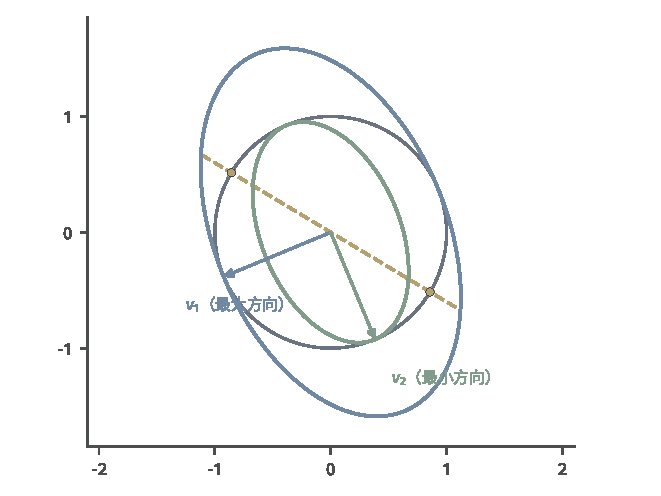
\includegraphics[width=112mm]{figures/00-shared/mathematical-preliminaries-upper/02-linear-spaces/matplotlib/ls-sphere-constrained-extremum/ls-sphere-constrained-extremum.pdf}
  \caption{单位圆约束下的极值落在特征方向。$\bm S=\left[\begin{smallmatrix}2&0.5\\0.5&1\end{smallmatrix}\right]$，
  灰圆为$\lVert\bm x\rVert=1$。蓝椭圆$\bm x^\top\bm S\bm x=\lambda_1\approx2.21$在
  $\pm\bm v_1$处与单位圆相切（最大值），绿椭圆$=\lambda_2\approx0.79$在$\pm\bm v_2$处
  相切（最小值）；黄色虚线为子空间约束直线，其上黄点是该约束下的两个极值，
  第~\ref{sec:ls-spectral-value-sensitivity}节的最小最大原理使用这种限制。
  $\lambda_{1,2}=(3\pm\sqrt2)/2$。固定复算。}
  \label{fig:ls-sphere-constrained-extremum}
\end{figure}

回到开头的对角矩阵，现在可以完成全部单位方向的比较。

\begin{example}[对角矩阵在全部单位方向上的比较]
\label{ex:ls-rayleigh-diagonal-two-by-two}
取$\bm S=\operatorname{diag}(4,1)$。每个单位向量都能写成$\bm x=(\cos\theta,\sin\theta)^\top$，其中$\theta\in[0,2\pi)$，于是
\[
 \bm x^\top\bm S\bm x=4\cos^2\theta+\sin^2\theta=1+3\cos^2\theta .
\]
由$0\leq\cos^2\theta\leq1$，它介于$1$与$4$之间：$\cos^2\theta=1$即$\bm x=\pm\bm e_1$时取最大值$4$，$\cos^2\theta=0$即$\bm x=\pm\bm e_2$时取最小值$1$。$\theta=\pi/4$时$\cos^2\theta=1/2$，得到开头的$5/2$。

可见最大值$4$与最小值$1$正是两个特征值，取到它们的方向正是特征方向，与定理~\ref{thm:matrix-analysis-rayleigh-ritz}一致；倾斜方向的值都严格介于两者之间。
\end{example}

定理不要求$\bm S$半正定。二次型可以取负值，例如$\bm S=\operatorname{diag}(1,-2)$时
\[
 \bm x^\top\bm S\bm x=x_1^2-2x_2^2 ,
\]
单位方向上的值仍介于$-2$与$1$之间，两端分别在$\pm\bm e_2$与$\pm\bm e_1$取到。

\paragraph{最优方向的唯一性}
还要区分最优值与最优方向的唯一性。最大值$\lambda_1$总是唯一的数，取到它的方向则由特征空间$\ker(\bm S-\lambda_1\bm I)$决定。

$\lambda_1$单重时，这个空间是一条直线，单位最优方向只有$\pm\bm q_1$两个，相差一个符号。$\lambda_1$重复时，空间中每个单位向量都给出最大值，例如$\bm S=\bm I$时所有单位方向都是最优的。

重根时，谱分解中的$\bm q_1$只是最优方向中的一个代表，取决于特征基的选择；最优方向组成的集合则由定理~\ref{thm:ls-spectral-projections}唯一确定。最小值的情形相同。

\paragraph{特例：$\bm S=\bm A^\top\bm A$}
一个常见的特例是$\bm S=\bm A^\top\bm A$，其中$\bm A\in\mathbb R^{m\times d}$。这时
\[
 R_{\bm A^\top\bm A}(\bm x)=\frac{\bm x^\top\bm A^\top\bm A\bm x}{\bm x^\top\bm x}=\frac{\lVert\bm A\bm x\rVert_2^2}{\lVert\bm x\rVert_2^2},
\]
即输出长度与输入长度之比的平方。

第~\ref{chap:singular-value-decomposition}章已经说明$\bm A^\top\bm A$的特征值是奇异值的平方（$d>m$时补上零）。所以定理~\ref{thm:matrix-analysis-rayleigh-ritz}给出那里最大、最小输出长度的另一种解释：单位输入的输出长度最大为$\sigma_1$，在$\bm v_1$取到；最小为$\sqrt{\lambda_d}$，其中$\lambda_d$是$\bm A^\top\bm A$的最小特征值，在它的特征方向取到。

第~\ref{sec:linear-algebra-homogeneous-estimation}节的齐次最小二乘正是在单位输入中最小化这一量。若$\bm A$有非零的零空间，最小值为零，任一单位零空间向量都最优。若$\bm A$满列秩，则$\bm A\bm x\neq\bm0$对一切$\bm x\neq\bm0$成立，$\bm A^\top\bm A\succ0$，由定理~\ref{thm:ls-symmetric-definiteness-eigenvalues}，最小值为正。

\paragraph{回到秩一逼近}
现在取$\bm S=\bm G=\bm A\bm A^\top$。由定理~\ref{thm:matrix-analysis-rayleigh-ritz}，单位方向的保留量最大为$\lambda_1(\bm G)$，恰在$\ker(\bm G-\lambda_1(\bm G)\bm I)$中的单位向量处取到。代入式~\eqref{eq:matrix-approximation-rank-one-error}，最小平方误差为
\begin{equation}
 \min_{\operatorname{rank}\bm X\leq1}\lVert\bm A-\bm X\rVert_{\mathrm F}^2=\lVert\bm A\rVert_{\mathrm F}^2-\lambda_1(\bm G) .
 \label{eq:matrix-approximation-rank-one-min-error-gram}
\end{equation}

这里只使用了第~\ref{chap:eigen-spectral-decomposition}章已经证明的谱分解。谱分解的存在不依赖本节的极值结论，本节只是用它读出极值。

\begin{example}[比较两个特征方向]
\label{ex:matrix-approximation-rank-one-eigen-directions}
沿用示例~\ref{ex:matrix-approximation-rank-one-fixed-direction}的$\bm A$。$\bm G=\bm A\bm A^\top$的元素是$\bm A$两行的内积：
\[
 g_{11}=2^2+1^2=5,\qquad g_{12}=g_{21}=2\cdot1+1\cdot2=4,\qquad g_{22}=1^2+2^2=5,
\]
即
\[
 \bm G=\begin{bmatrix}5&4\\4&5\end{bmatrix}.
\]

逐行相乘可以验证两个特征向量：
\[
 \bm G\begin{bmatrix}1\\1\end{bmatrix}=\begin{bmatrix}5+4\\4+5\end{bmatrix}=9\begin{bmatrix}1\\1\end{bmatrix},\qquad
 \bm G\begin{bmatrix}1\\-1\end{bmatrix}=\begin{bmatrix}5-4\\4-5\end{bmatrix}=\begin{bmatrix}1\\-1\end{bmatrix}.
\]
所以两个标准正交特征方向$(1,1)^\top/\sqrt2$与$(1,-1)^\top/\sqrt2$的保留量分别是$9$与$1$，重建平方误差分别是$10-9=1$与$10-1=9$。

也可以直接比较全部单位方向。取$\bm u=(\cos\theta,\sin\theta)^\top$，
\[
 \bm u^\top\bm G\bm u=5\cos^2\theta+8\cos\theta\sin\theta+5\sin^2\theta=5+4\sin2\theta ,
\]
它介于$1$与$9$之间，在$\theta=\pi/4$与$\theta=3\pi/4$分别取到最大与最小值；$\theta=0$即$\bm u=\bm e_1$时为$5$，与示例~\ref{ex:matrix-approximation-rank-one-fixed-direction}末尾的比较一致。

所以那里所取的方向$(1,1)^\top/\sqrt2$已是最优方向，而$(1,-1)^\top/\sqrt2$是最差的方向。
\end{example}

\subsection{最优解与逼近误差}
\label{sec:matrix-approximation-rank-one-solution}

\paragraph{由奇异值分解读出最优解}
上一小节用$\bm G$的特征方向给出了最优直线，现在把它与$\bm A$的奇异值分解联系起来，写出最优近似矩阵。设$\bm A\neq\bm0$，奇异值为$\sigma_1\geq\cdots\geq\sigma_r>0$。

式~\eqref{eq:ls-svd-transpose-relation}说明，$\bm G=\bm A\bm A^\top$的特征值是$\sigma_1^2,\ldots,\sigma_r^2$及$m-r$个零，左奇异向量$\bm u_i$是对应的特征向量。因此最大保留量为$\lambda_1(\bm G)=\sigma_1^2$，取$\bm u=\bm u_1$即可达到。

总平方长度也由奇异值给出：
\[
 \lVert\bm A\rVert_{\mathrm F}^2=\operatorname{tr}\bm G=\sum_{i=1}^r\sigma_i^2 .
\]
所以最小平方误差为
\begin{equation}
 \lVert\bm A\rVert_{\mathrm F}^2-\sigma_1^2=\sum_{i=2}^r\sigma_i^2 .
 \label{eq:matrix-approximation-rank-one-min-error}
\end{equation}

再求最优系数。由式~\eqref{eq:ls-svd-transpose-relation}，$\bm A^\top\bm u_1=\sigma_1\bm v_1$，所以
\[
 \bm c=\bm A^\top\bm u_1=\sigma_1\bm v_1 .
\]
把最佳方向与最优系数合成：
\begin{equation}
 \bm A_1=\bm u_1\bm u_1^\top\bm A=\bm u_1(\bm A^\top\bm u_1)^\top=\sigma_1\bm u_1\bm v_1^\top .
 \label{eq:matrix-approximation-rank-one-optimum}
\end{equation}

这是原矩阵$\bm A$的秩一近似，即和式~\eqref{eq:matrix-analysis-svd-rank-one-sum}的第一项，而不是Gram矩阵$\bm G$的秩一近似。计算的输入是$\bm A$，输出是近似矩阵$\bm A_1$；它不是某个方程的解向量。

\paragraph{计算步骤}
按上面的推导，计算秩一最优逼近只需三件事：求出保留量最大的方向，求出各列在该方向上的系数，再把两者合成。下面写出用到的变量与步骤，并用以下数据逐步演示：
\[
 \bm A=\begin{bmatrix}2&1\\1&2\end{bmatrix}.
\]
这是示例~\ref{ex:matrix-approximation-rank-one-fixed-direction}的矩阵。

变量如下。
\begin{itemize}
 \item $\sigma_1^2$与$\bm u_1\in\mathbb R^m$：$\bm G=\bm A\bm A^\top$的最大特征值与一个单位特征向量，即最大保留量与最优方向。
 \item $\bm c\in\mathbb R^d$：各列在$\bm u_1$上的投影系数，等于$\sigma_1\bm v_1$。
 \item $\bm A_1\in\mathbb R^{m\times d}$：秩一近似矩阵。
 \item $e$：平方误差$\lVert\bm A-\bm A_1\rVert_{\mathrm F}^2$，用于核对。
\end{itemize}

依次执行以下步骤。
\begin{enumerate}
 \item \textbf{求最优方向。}求$\bm G=\bm A\bm A^\top$的最大特征值$\sigma_1^2$与单位特征向量$\bm u_1$；若已有$\bm A$的奇异值分解，直接读出$\sigma_1$与$\bm u_1$。例中示例~\ref{ex:matrix-approximation-rank-one-eigen-directions}已求得
 \[
  \sigma_1^2=9,\qquad \bm u_1=\frac1{\sqrt2}\begin{bmatrix}1\\1\end{bmatrix}.
 \]

 \item \textbf{求系数。}按式~\eqref{eq:matrix-approximation-rank-one-coefficients}计算
 \[
  \bm c=\bm A^\top\bm u_1 .
 \]
 例中
 \[
  \bm c=\frac1{\sqrt2}\begin{bmatrix}2+1\\1+2\end{bmatrix}=\frac3{\sqrt2}\begin{bmatrix}1\\1\end{bmatrix}.
 \]
 它等于$\sigma_1\bm v_1$，其中$\sigma_1=3$、$\bm v_1=(1,1)^\top/\sqrt2$；已有奇异值分解时这一步可直接取$\sigma_1\bm v_1$。

 \item \textbf{合成近似矩阵。}按式~\eqref{eq:matrix-approximation-rank-one-optimum}作外积
 \[
  \bm A_1=\bm u_1\bm c^\top .
 \]
 例中
 \[
  \bm A_1=\frac1{\sqrt2}\cdot\frac3{\sqrt2}\begin{bmatrix}1&1\\1&1\end{bmatrix}=\frac32\begin{bmatrix}1&1\\1&1\end{bmatrix}.
 \]

 \item \textbf{核对误差。}求残差$\bm A-\bm A_1$的平方和，并与$\lVert\bm A\rVert_{\mathrm F}^2-\sigma_1^2$比较。例中
 \[
  \bm A-\bm A_1=\frac12\begin{bmatrix}1&-1\\-1&1\end{bmatrix},\qquad
  e=1=10-9 .
 \]
\end{enumerate}

最终得到
\[
 \bm A_1=\frac32\begin{bmatrix}1&1\\1&1\end{bmatrix}.
\]
它的四个元素都是$3/2$，两列成比例，秩为一。另一个奇异值是$\sigma_2=1$（$\bm A(1,-1)^\top=(1,-1)^\top$），平方误差$1=\sigma_2^2$，与最小误差公式一致。

同样的步骤用于示例~\ref{ex:ls-low-rank-three-columns}。这时$\bm G=\operatorname{diag}(9,4,1)$，最大特征值为$9$，$\bm u_1=\bm e_1$。系数与合成的近似矩阵为
\[
 \bm c=\bm A^\top\bm e_1=\begin{bmatrix}3\\0\\0\end{bmatrix},\qquad \bm A_1=3\bm e_1\bm e_1^\top .
\]
它只保留第一列，另两列被投影成零，平方误差为
\[
 14-9=5=4+1 .
\]

\paragraph{列重建与行重建}
这里用的是$\bm A\bm A^\top$而不是$\bm A^\top\bm A$，因为我们重建的是$\mathbb R^m$中的列向量。保留量直接等于列向量在$\bm u$上的投影长度平方之和，对应的是左奇异方向。

若改为重建行向量，同样的推导会用到$\bm A^\top\bm A$与右奇异方向$\bm v_1$。由$\bm A\bm v_1=\sigma_1\bm u_1$，得到的近似是
\[
 \bm A\bm v_1\bm v_1^\top=\sigma_1\bm u_1\bm v_1^\top ,
\]
与式~\eqref{eq:matrix-approximation-rank-one-optimum}是同一个矩阵。

这种解释依赖$\bm G$是Gram矩阵。对一般不定的对称矩阵$\bm S$，二次型值可能为负，不能把任意Rayleigh商的极值都解释成某个矩阵的最佳秩一逼近。

\paragraph{最优矩阵的唯一性}
最后区分最优近似矩阵与它的表示。$\bm A=\bm0$时$r=0$，每个方向的保留量都是零，唯一的最优近似是零矩阵。

$\sigma_1>\sigma_2$（或$r=1$）时，$\bm G$最大特征值的特征空间是一条直线，最优方向只有$\pm\bm u_1$。把$(\bm u_1,\bm v_1)$同时换成$(-\bm u_1,-\bm v_1)$不改变外积，所以最优矩阵$\bm A_1$唯一，不唯一的只是它的写法。

$\sigma_1=\sigma_2$时情况不同：最大特征值的特征空间至少二维，其中每个单位向量$\bm u$都给出最优近似$\bm u\bm u^\top\bm A$，不同的直线给出不同的矩阵。例如$\bm A=\bm I_2$时，$\bm G=\bm I_2$，每个单位向量$\bm u$的保留量都是$1$，误差都是
\[
 \lVert\bm I_2-\bm u\bm u^\top\rVert_{\mathrm F}^2=2-1=1 ;
\]
$\bm e_1\bm e_1^\top$与$\bm e_2\bm e_2^\top$就是两个不同的最优近似。

所以表示的非唯一性不等于近似矩阵的非唯一性，后者只来自最大奇异值重复。下一步保持误差标准不变，把允许保留的方向数由一个增加到$k$个。

% 第15章第3节：秩k逼近（子空间选择与迹极值、截断SVD的构造、最佳误差与最优性、最优解的唯一性）。

\section{秩\texorpdfstring{$k$}{k}逼近}
\label{sec:ls-low-rank-approximation}
\label{sec:ls-low-rank-solve}
\label{sec:ls-full-svd-solve}
\label{sec:matrix-analysis-svd-low-rank}

把共同的重建方向由一条直线扩展为$k$维子空间。与秩一情形一样，先固定子空间求系数，再选择子空间本身；用子空间的标准正交基，保留量写成一个迹，选子空间就成为迹的极值问题。由奇异值分解可以写出这个问题的解，即截断SVD；随后在Frobenius范数与谱范数下证明它的最优性，并讨论最优解何时唯一。

\subsection{子空间选择与迹极值}
\label{sec:ls-low-rank-projection-error}
\label{sec:ls-rank-k-trace}

\paragraph{固定子空间时的最优重建}
秩约束要求全部重建向量共用至多$k$个独立方向。先把这些方向张成的$k$维子空间固定下来，问每一列应当怎样重建。直观上，答案应当是把每一列正交投影到这个子空间上，这与秩一情形相同；下面把这一点写成等式。

以列标准正交的$\bm Y\in\mathbb R^{m\times k}$表示这个子空间，
\[
 \bm Y^\top\bm Y=\bm I_k ;
\]
这里不用字母$\bm V$，以免与右奇异向量矩阵混淆。列都落在$\operatorname{range}(\bm Y)$中的矩阵恰好是
\[
 \bm X=\bm Y\bm C,\qquad \bm C\in\mathbb R^{k\times d},
\]
$\bm C$的第$j$列是$\bm x_j$在这组基下的系数。由第~\ref{chap:inner-product-spaces}章的投影矩阵，$\bm Y\bm Y^\top$是到$\operatorname{range}(\bm Y)$的正交投影。

以$m=3$、$k=2$、$\bm Y=[\bm e_1,\bm e_2]$为例，按元素写出
\[
 \begin{gathered}
 \bm Y\bm Y^\top=\begin{bmatrix}1&0&0\\0&1&0\\0&0&0\end{bmatrix},\\
 \bm Y\bm C=\begin{bmatrix}c_{1,1}&\cdots&c_{1,d}\\c_{2,1}&\cdots&c_{2,d}\\0&\cdots&0\end{bmatrix}.
 \end{gathered}
\]
投影保留每一列的前两个分量、去掉第三个分量；候选矩阵的第三行只能是零，前两行可以任意选取。

\begin{lemma}[固定子空间时的正交误差分解]
\label{lem:ls-low-rank-projection-error}
设$\bm Y\in\mathbb R^{m\times k}$满足$\bm Y^\top\bm Y=\bm I_k$，则对任意$\bm C\in\mathbb R^{k\times d}$，
\begin{equation}
 \begin{aligned}
 \lVert\bm A-\bm Y\bm C\rVert_{\mathrm F}^2
 &=\lVert(\bm I-\bm Y\bm Y^\top)\bm A\rVert_{\mathrm F}^2\\
 &\qquad+\lVert\bm Y^\top\bm A-\bm C\rVert_{\mathrm F}^2,
 \end{aligned}
 \label{eq:ls-low-rank-projection-split}
\end{equation}
并且
\begin{equation}
 \lVert(\bm I-\bm Y\bm Y^\top)\bm A\rVert_{\mathrm F}^2
 =\lVert\bm A\rVert_{\mathrm F}^2-\operatorname{tr}(\bm Y^\top\bm A\bm A^\top\bm Y).
 \label{eq:ls-low-rank-projection-residual}
\end{equation}
因此固定子空间时，最优系数唯一，为$\bm C=\bm Y^\top\bm A$，最优重建是正交投影$\bm Y\bm Y^\top\bm A$。
\end{lemma}
\begin{proof}
把误差矩阵拆成两部分：
\[
 \bm A-\bm Y\bm C=(\bm I-\bm Y\bm Y^\top)\bm A+\bm Y(\bm Y^\top\bm A-\bm C).
\]
逐列看，第$j$列是$\bm r_j=(\bm I-\bm Y\bm Y^\top)\bm a_j$与$\bm Y\bm z_j$之和，其中$\bm z_j$是$\bm Y^\top\bm A-\bm C$的第$j$列。二者正交：
\[
 \bm r_j^\top\bm Y\bm z_j=\bm a_j^\top(\bm I-\bm Y\bm Y^\top)\bm Y\bm z_j
 =\bm a_j^\top(\bm Y-\bm Y\bm Y^\top\bm Y)\bm z_j=0 ,
\]
这里用到$\bm Y^\top\bm Y=\bm I_k$。又由同一关系，
\[
 \lVert\bm Y\bm z_j\rVert_2^2=\bm z_j^\top\bm Y^\top\bm Y\bm z_j=\lVert\bm z_j\rVert_2^2 .
\]
由勾股定理，误差矩阵第$j$列的平方长度是
\[
 \lVert\bm r_j\rVert_2^2+\lVert\bm z_j\rVert_2^2 ;
\]
对$j$求和即得式~\eqref{eq:ls-low-rank-projection-split}。

对第二式，同样把$\bm a_j$分解为$\bm Y\bm Y^\top\bm a_j$与$\bm r_j$两个正交部分，得
\[
 \lVert\bm r_j\rVert_2^2=\lVert\bm a_j\rVert_2^2-\lVert\bm Y^\top\bm a_j\rVert_2^2 .
\]
求和后，
\[
 \sum_j\lVert\bm Y^\top\bm a_j\rVert_2^2=\lVert\bm Y^\top\bm A\rVert_{\mathrm F}^2
 =\operatorname{tr}(\bm Y^\top\bm A\bm A^\top\bm Y).
\]
最后，式~\eqref{eq:ls-low-rank-projection-split}右端第一项与$\bm C$无关，第二项非负，且当且仅当$\bm C=\bm Y^\top\bm A$时为零。
\end{proof}

于是在固定子空间中，误差等于总平方长度减去保留量$\operatorname{tr}(\bm Y^\top\bm A\bm A^\top\bm Y)$；$k=1$、$\bm Y=\bm u$时，这正是第~\ref{sec:matrix-approximation-rank-one-coefficients}节逐列配方得到的公式。示例~\ref{ex:ls-low-rank-three-columns}中“先投影再计损失”的做法，也正是这个最优重建。

共同子空间把$d$个向量各自的最小二乘问题合成了一个矩阵近似问题：子空间共用，系数逐列由投影给出。

在上面$\bm Y=[\bm e_1,\bm e_2]$的例子中，取$\bm A=\operatorname{diag}(3,2,1)$，最优系数与最优重建为
\[
 \begin{gathered}
 \bm Y^\top\bm A=\begin{bmatrix}3&0&0\\0&2&0\end{bmatrix},\\
 \bm Y\bm Y^\top\bm A=\begin{bmatrix}3&0&0\\0&2&0\\0&0&0\end{bmatrix}.
 \end{gathered}
\]
残差只剩右下角的$1$，平方误差为
\[
 \lVert\bm A\rVert_{\mathrm F}^2-\operatorname{tr}(\bm Y^\top\bm A\bm A^\top\bm Y)=14-(9+4)=1 ,
\]
与示例~\ref{ex:ls-low-rank-three-columns}中坐标平面$\operatorname{span}\{\bm e_1,\bm e_2\}$的损失一致。

\paragraph{化为子空间的选择}
引理只处理了列都落在给定子空间中的候选。下面说明，这一化归覆盖全部秩不超过$k$的矩阵，而不只覆盖事先写成投影形式的矩阵。

设$\operatorname{rank}\bm X=s\leq k$。取$\bm X$列空间的一组标准正交基，再在$\mathbb R^m$中补充$k-s$个与之正交的单位向量（$k\leq m$，所以可以补齐），排成$\bm Y$。则$\bm X$的列都落在$\operatorname{range}(\bm Y)$中，
\[
 \bm X=\bm Y\bm C,\qquad \bm C=\bm Y^\top\bm X .
\]
由引理~\ref{lem:ls-low-rank-projection-error}，
\[
 \lVert\bm A-\bm X\rVert_{\mathrm F}^2\geq\lVert\bm A\rVert_{\mathrm F}^2-\operatorname{tr}(\bm Y^\top\bm A\bm A^\top\bm Y).
\]
反过来，每个列标准正交的$\bm Y$都给出秩不超过$k$的候选$\bm Y\bm Y^\top\bm A$，误差恰为右端。两方面合起来，
\begin{equation}
 \begin{aligned}
 &\min_{\operatorname{rank}\bm X\leq k}\lVert\bm A-\bm X\rVert_{\mathrm F}^2\\
 &\qquad=\lVert\bm A\rVert_{\mathrm F}^2-\max_{\bm Y^\top\bm Y=\bm I_k}\operatorname{tr}(\bm Y^\top\bm A\bm A^\top\bm Y),
 \end{aligned}
 \label{eq:ls-low-rank-subspace-reduction}
\end{equation}
只要右端的最大值存在；最大值的存在与取值由下面的定理~\ref{thm:matrix-analysis-trace-minimum}给出。到这里，“同时选择方向与系数”化成了“选择子空间”。

\paragraph{保留量的含义}
再看保留量本身。对$\bm Y=[\bm y_1,\ldots,\bm y_k]$按列展开：
\[
 \begin{aligned}
 \operatorname{tr}(\bm Y^\top\bm A\bm A^\top\bm Y)
 &=\sum_{l=1}^k\bm y_l^\top\bm A\bm A^\top\bm y_l\\
 &=\sum_{l=1}^k\sum_{j=1}^d(\bm y_l^\top\bm a_j)^2 .
 \end{aligned}
\]
迹把$k$个互相垂直方向上的保留量相加，$k=1$时恰好回到上一节的Rayleigh商。

保留量只依赖子空间，不依赖基的选取。记$\bm G=\bm A\bm A^\top$。把$\bm Y$换成$\bm Y\bm O$（$\bm O$为$k$阶正交矩阵）时，由迹的循环性，
\[
 \operatorname{tr}(\bm O^\top\bm Y^\top\bm G\bm Y\bm O)=\operatorname{tr}(\bm Y^\top\bm G\bm Y).
\]

据此，由式~\eqref{eq:ls-low-rank-subspace-reduction}，秩$k$逼近归结为下面的\emph{迹极值问题}：
\[
 \begin{gathered}
 \text{在}\ \bm Y^\top\bm Y=\bm I_k\ \text{下最大化}\ \operatorname{tr}(\bm Y^\top\bm G\bm Y),\\
 \bm G=\bm A\bm A^\top .
 \end{gathered}
\]

\paragraph{两个候选界}
逐列套用Rayleigh--Ritz定理只能得到每一项不超过$\lambda_1(\bm G)$，即
\[
 \operatorname{tr}(\bm Y^\top\bm G\bm Y)\leq k\lambda_1(\bm G).
\]
这个界没有用到各列互相正交的约束，一般取不到：由定理~\ref{thm:matrix-analysis-rayleigh-ritz}的取等条件，总和等于$k\lambda_1(\bm G)$要求每个$\bm y_l$都落在最大特征值的特征空间中；若$\lambda_1(\bm G)$单重，这个特征空间是一条直线，$k\geq2$时容不下$k$个互相正交的单位向量。

另一个方向是只比较由$\bm G$的特征向量组成的子空间。设$\bm G$的特征值为$\lambda_1\geq\cdots\geq\lambda_m$，对应标准正交特征向量$\bm q_1,\ldots,\bm q_m$。取$\bm Y=[\bm q_{i_1},\ldots,\bm q_{i_k}]$（下标互不相同），则$\bm y_l^\top\bm G\bm y_l=\lambda_{i_l}$，保留量为
\[
 \operatorname{tr}(\bm Y^\top\bm G\bm Y)=\lambda_{i_1}+\cdots+\lambda_{i_k}.
\]
保留前$k$个特征方向给出最大的特征值和$\sum_{i\leq k}\lambda_i$。

回到示例~\ref{ex:ls-low-rank-three-columns}，$\bm G=\operatorname{diag}(9,4,1)$。第一个界给出$2\times9=18$，超过总长度平方$14$，显然太松。三个坐标平面给出$13,10,5$，其中前两个特征方向张成的$\operatorname{span}\{\bm e_1,\bm e_2\}$最好，保留$13$、损失$1$。

一般地，由式~\eqref{eq:ls-svd-transpose-relation}，$\bm A\bm A^\top$的前$k$个特征方向可以取为左奇异向量$\bm u_1,\ldots,\bm u_k$，候选子空间就是$\operatorname{span}\{\bm u_1,\ldots,\bm u_k\}$。

\paragraph{倾斜子空间与权重}
任意倾斜的子空间会把权重分散到多个特征方向上，它是否仍不能超过特征值和，需要看清正交约束对权重的限制。仍取$\bm G=\operatorname{diag}(9,4,1)$，考虑倾斜平面
\[
 \bm Y=\begin{bmatrix}1&0\\0&1/\sqrt2\\0&1/\sqrt2\end{bmatrix}.
\]
它在三个特征方向$\bm e_1,\bm e_2,\bm e_3$上的权重$w_i=\lVert\bm Y^\top\bm e_i\rVert_2^2$依次是$\bm Y$各行的平方长度：
\[
 w_1=1,\qquad w_2=\frac12,\qquad w_3=\frac12 .
\]
保留量就是特征值的加权和：
\[
 \operatorname{tr}(\bm Y^\top\bm G\bm Y)=9\cdot1+4\cdot\frac12+1\cdot\frac12=\frac{23}2<13 .
\]
权重各不超过$1$，总和为$k=2$。这个平面把第二个特征方向上的一半权重让给了较小的第三个特征值，因而保留得更少。

下面的定理说明这对任意实对称矩阵、任意$k$维子空间都成立；同时也回答迹能否低于后$k$个特征值之和。

\begin{theorem}[迹极值]
\label{thm:matrix-analysis-trace-minimum}
设$\bm S\in\mathbb R^{m\times m}$实对称，特征值$\lambda_1\geq\cdots\geq\lambda_m$，对应标准正交特征向量$\bm q_1,\ldots,\bm q_m$，$1\leq k\leq m$。对满足$\bm Y^\top\bm Y=\bm I_k$的$\bm Y\in\mathbb R^{m\times k}$，
\begin{equation}
 \sum_{i=m-k+1}^{m}\lambda_i\leq\operatorname{tr}(\bm Y^\top\bm S\bm Y)\leq\sum_{i=1}^{k}\lambda_i,
 \label{eq:matrix-analysis-trace-minimum}
\end{equation}
上界由$\bm Y=[\bm q_1,\ldots,\bm q_k]$取到，下界由$\bm Y=[\bm q_{m-k+1},\ldots,\bm q_m]$取到。若$k<m$且$\lambda_k>\lambda_{k+1}$，则上界取等当且仅当$\operatorname{range}(\bm Y)=\operatorname{span}\{\bm q_1,\ldots,\bm q_k\}$。
\end{theorem}
\begin{proof}
由谱定理，$\bm S=\sum_i\lambda_i\bm q_i\bm q_i^\top$，故
\[
 \operatorname{tr}(\bm Y^\top\bm S\bm Y)
 =\sum_{i=1}^m\lambda_i\operatorname{tr}(\bm Y^\top\bm q_i\bm q_i^\top\bm Y)
 =\sum_{i=1}^m\lambda_iw_i,
\]
其中$w_i=\lVert\bm Y^\top\bm q_i\rVert_2^2$。权重受两条限制。

第一，$\bm P=\bm Y\bm Y^\top$是到$\operatorname{range}(\bm Y)$的正交投影，满足$\bm P=\bm P^\top\bm P$，所以
\[
 w_i=\bm q_i^\top\bm P\bm q_i=\bm q_i^\top\bm P^\top\bm P\bm q_i=\lVert\bm P\bm q_i\rVert_2^2 .
\]
正交投影不增加长度，所以$0\leq w_i\leq\lVert\bm q_i\rVert_2^2=1$。

第二，记$\bm Q=[\bm q_1,\ldots,\bm q_m]$，它是正交矩阵，右乘正交矩阵不改变Frobenius范数，于是
\[
 \sum_{i=1}^mw_i=\lVert\bm Y^\top\bm Q\rVert_{\mathrm F}^2=\lVert\bm Y^\top\rVert_{\mathrm F}^2=\operatorname{tr}(\bm Y^\top\bm Y)=k .
\]
也就是说，总量为$k$的权重分配给各个特征值，每个特征值至多分到$1$。

直观上，要使加权和最大，应把权重全部放在最大的$k$个特征值上。用$\lambda_k$作为分界，可以把这一直观写成恒等式：
\[
 \begin{aligned}
 \sum_{i=1}^m\lambda_iw_i-\sum_{i=1}^k\lambda_i
 &=\sum_{i\leq k}(\lambda_i-\lambda_k)(w_i-1)+\sum_{i>k}(\lambda_i-\lambda_k)w_i\\
 &\qquad+\lambda_k\Bigl(\sum_{i=1}^mw_i-k\Bigr).
 \end{aligned}
\]
展开右端即可核对。最后一项因$\sum_iw_i=k$而为零。$i\leq k$时$\lambda_i-\lambda_k\geq0$、$w_i-1\leq0$；$i>k$时$\lambda_i-\lambda_k\leq0$、$w_i\geq0$。所以右端每一项都不大于零，上界成立。

上界可以取到：$\bm Y=[\bm q_1,\ldots,\bm q_k]$时$w_i$在$i\leq k$时为$1$、其余为$0$，迹等于$\sum_{i\leq k}\lambda_i$。

取等条件也可以从这个恒等式读出。若$\lambda_k>\lambda_{k+1}$，则$i>k$时$\lambda_i-\lambda_k<0$，上界取等迫使$w_i=0$，即$\bm Y^\top\bm q_i=\bm0$。于是$\operatorname{range}(\bm Y)$与$\bm q_{k+1},\ldots,\bm q_m$都正交，含于$\operatorname{span}\{\bm q_1,\ldots,\bm q_k\}$；两者都是$k$维的，所以相等。

反之，若$\operatorname{range}(\bm Y)=\operatorname{span}\{\bm q_1,\ldots,\bm q_k\}$，则$i\leq k$时$\bm P\bm q_i=\bm q_i$、$i>k$时$\bm P\bm q_i=\bm0$，迹等于上界。

下界由上界得到。$-\bm S$的特征值按降序为$-\lambda_m\geq\cdots\geq-\lambda_1$，对应特征向量依次为$\bm q_m,\ldots,\bm q_1$。对$-\bm S$应用上界，得
\[
 -\operatorname{tr}(\bm Y^\top\bm S\bm Y)\leq-\sum_{i=m-k+1}^m\lambda_i ,
\]
等号在$\bm Y=[\bm q_{m-k+1},\ldots,\bm q_m]$时成立。
\end{proof}

在倾斜平面的例子中，恒等式右端的三类项分别是
\[
 (9-4)(1-1)=0,\qquad (4-4)\Bigl(\frac12-1\Bigr)=0,\qquad (1-4)\cdot\frac12=-\frac32 .
\]
合计$-\tfrac32$，正是$\tfrac{23}2-13$：亏损全部来自让给第三个特征值的那一半权重。

\paragraph{回到低秩逼近}
取$\bm S=\bm G=\bm A\bm A^\top$。它的特征值是$\sigma_1^2\geq\cdots\geq\sigma_r^2$，再补上$m-r$个零；$k<r$时前$k$个之和为$\sum_{i\leq k}\sigma_i^2$。于是任意$k$维子空间最多保留
\begin{equation}
 \max_{\bm Y^\top\bm Y=\bm I_k}\operatorname{tr}(\bm Y^\top\bm A\bm A^\top\bm Y)=\sum_{i=1}^k\sigma_i^2 ,
 \label{eq:ls-low-rank-max-retained}
\end{equation}
式~\eqref{eq:ls-low-rank-subspace-reduction}右端的最大值存在，并由$\operatorname{span}\{\bm u_1,\ldots,\bm u_k\}$取到。在示例~\ref{ex:ls-low-rank-three-columns}中，这确认任意倾斜平面的保留量都不超过$13$，坐标平面$\operatorname{span}\{\bm e_1,\bm e_2\}$已是最优的平面。

对一般的对称矩阵$\bm S$，迹极值界照样成立，但只有在当前这种半正定的Gram情形，迹才表示投影保留的长度平方。下一小节把最优子空间上的投影重建写成具体的矩阵。

\subsection{截断SVD的构造}
\label{sec:ls-truncated-svd-construction}

\subsubsection{主要思想}

上一小节确定了最优子空间，还没有写出最优重建本身。设$\bm A$的奇异值分解写成和式~\eqref{eq:matrix-analysis-svd-rank-one-sum}，
\[
 \bm A=\sum_{i=1}^r\sigma_i\bm u_i\bm v_i^\top ,
\]
其中$r=\operatorname{rank}\bm A$，$\sigma_1\geq\cdots\geq\sigma_r>0$。$1\leq k<r$时最优子空间可取为$\operatorname{span}\{\bm u_1,\ldots,\bm u_k\}$，即
\[
 \bm Y=\bm U_k=[\bm u_1,\ldots,\bm u_k].
\]
由引理~\ref{lem:ls-low-rank-projection-error}，最优重建是$\bm U_k\bm U_k^\top\bm A$。要把它化简，只需看$\bm U_k^\top$作用在每个$\bm u_i$上的结果。

以$r=3$、$k=2$为例，由$\bm u_i$标准正交，按元素写出
\[
 \bm U_2^\top\bm u_1=\begin{bmatrix}1\\0\end{bmatrix},\qquad
 \bm U_2^\top\bm u_2=\begin{bmatrix}0\\1\end{bmatrix},\qquad
 \bm U_2^\top\bm u_3=\begin{bmatrix}0\\0\end{bmatrix}.
\]
于是$\bm U_2\bm U_2^\top\bm u_i$在$i=1,2$时还原为$\bm u_i$，在$i=3$时为零。一般地，$\bm U_k^\top\bm u_i$在$i\leq k$时等于$\bm e_i$、在$i>k$时等于$\bm0$，所以
\[
 \begin{aligned}
 \bm U_k\bm U_k^\top\bm A
 &=\sum_{i=1}^r\sigma_i\bm U_k(\bm U_k^\top\bm u_i)\bm v_i^\top\\
 &=\sum_{i=1}^k\sigma_i\bm u_i\bm v_i^\top .
 \end{aligned}
\]
也就是说，把$\bm A$的各列正交投影到前$k$个左奇异方向上，等于只保留SVD和式的前$k$项。

把这个由子空间优化推导出的矩阵记下来。对整数$k\geq0$，称
\begin{equation}
\begin{gathered}
\bm A_k=\sum_{i=1}^{\min(k,r)}\sigma_i\bm u_i\bm v_i^\top
 =\bm U_k\bm\Sigma_k\bm V_k^\top\\
k\geq0
\end{gathered}
\label{eq:matrix-analysis-truncated-svd}
\end{equation}
为$\bm A$的\term{截断SVD}（truncated SVD），其中$k\leq r$时$\bm\Sigma_k=\operatorname{diag}(\sigma_1,\ldots,\sigma_k)$，$\bm V_k=[\bm v_1,\ldots,\bm v_k]$。两种边界情形与第~\ref{sec:matrix-approximation-problem}节的直接回答一致：$k=0$时和式为空，$\bm A_0=\bm0$；$k\geq r$时保留了全部项，$\bm A_k=\bm A$。

$\bm A_k$满足秩约束。$k\leq r$时，
\[
 \bm A_k\bm v_i=\sigma_i\bm u_i\quad(i\leq k),\qquad
 \bm A_k\bm v_i=\bm0\quad(i>k),
\]
所以列空间恰为$\operatorname{span}\{\bm u_1,\ldots,\bm u_k\}$，$\operatorname{rank}\bm A_k=k$。

\subsubsection{算法实现}

截断SVD的输入是$\bm A$已经求出的SVD与秩预算$k$，输出是$\bm A_k$或它的三个因子。计算本身不迭代：取出前$k$组奇异值与奇异向量，相乘即可。下面用以下示例中的矩阵逐步演示；它的一个奇异方向是倾斜的，并且有重奇异值。

\begin{example}[有重奇异值的三阶截断]
\label{ex:matrix-approximation-truncated-three-by-three}
取
\[
 \bm A=\begin{bmatrix}3&2&0\\2&3&0\\0&0&1\end{bmatrix}.
\]
令
\[
 \bm u_1=\frac1{\sqrt2}\begin{bmatrix}1\\1\\0\end{bmatrix},\qquad
 \bm u_2=\frac1{\sqrt2}\begin{bmatrix}1\\-1\\0\end{bmatrix},\qquad
 \bm u_3=\begin{bmatrix}0\\0\\1\end{bmatrix},
\]
它们标准正交，且
\[
 \bm A\bm u_1=5\bm u_1,\qquad\bm A\bm u_2=\bm u_2,\qquad\bm A\bm u_3=\bm u_3 .
\]
$\bm A$对称、特征值非负，所以可取$\bm v_i=\bm u_i$，奇异值为$5,1,1$。下面分别取$k=1$与$k=2$。
\end{example}

\paragraph{变量}
\begin{itemize}
 \item $k$：秩预算；$r$：$\bm A$的秩，即正奇异值的个数。
 \item $\sigma_i,\bm u_i,\bm v_i$：已经求出的奇异值与配对的左右奇异向量。
 \item $\bm U_k\in\mathbb R^{m\times k}$、$\bm\Sigma_k$、$\bm V_k\in\mathbb R^{d\times k}$：截取出的三个因子。
 \item $\bm W=\bm\Sigma_k\bm V_k^\top\in\mathbb R^{k\times d}$：缩放后的右因子，即最优系数矩阵。
 \item $\bm A_k$：截断SVD；$\bm E_k=\bm A-\bm A_k$：重建残差，只在核验时形成。
\end{itemize}

\paragraph{输入与预处理}
先核对$k$是满足$0\leq k\leq\min(m,d)$的整数，并由正奇异值的个数确定$r$。$k=0$时直接输出零矩阵；$k\geq r$时直接输出$\bm A$。其余情形下，确认奇异值按非增顺序排列；若SVD例程给出的顺序不同，就把奇异值连同配对的左右奇异向量一起重新排序。配对不能打乱，因为每一项$\sigma_i\bm u_i\bm v_i^\top$都要求$\bm A\bm v_i=\sigma_i\bm u_i$。

例中$r=3$，$k=1,2$都满足$1\leq k<r$，奇异值$5,1,1$已按非增顺序排列。

\paragraph{计算步骤}
\begin{enumerate}
 \item \textbf{截取因子。}取前$k$组奇异值与奇异向量，
 \[
  \bm U_k=[\bm u_1,\ldots,\bm u_k],\qquad
  \bm\Sigma_k=\operatorname{diag}(\sigma_1,\ldots,\sigma_k),
 \]
 $\bm V_k=[\bm v_1,\ldots,\bm v_k]$。若只需要压缩存储，到这一步即可输出三个因子，不必形成$m\times d$的矩阵。

 例中$k=1$时$\bm U_1=\bm V_1=\bm u_1$，$\bm\Sigma_1=5$；$k=2$时
 \[
  \bm U_2=\bm V_2=\frac1{\sqrt2}\begin{bmatrix}1&1\\1&-1\\0&0\end{bmatrix},\qquad
  \bm\Sigma_2=\begin{bmatrix}5&0\\0&1\end{bmatrix}.
 \]

 \item \textbf{缩放右因子。}把$\bm V_k^\top$的第$i$行乘以$\sigma_i$：
 \begin{equation}
  \bm W=\bm\Sigma_k\bm V_k^\top .
  \label{eq:ls-truncated-svd-coefficients}
 \end{equation}
 由$\bm A^\top\bm u_i=\sigma_i\bm v_i$，$\bm W=\bm U_k^\top\bm A$，它正是引理~\ref{lem:ls-low-rank-projection-error}中的最优系数。

 例中$k=2$时
 \[
  \bm W=\frac1{\sqrt2}\begin{bmatrix}5&5&0\\1&-1&0\end{bmatrix},
 \]
 第一行即$k=1$时的$\bm W$。

 \item \textbf{相乘重建。}按式~\eqref{eq:matrix-analysis-truncated-svd}计算
 \[
  \bm A_k=\bm U_k\bm W=\sum_{i=1}^k\sigma_i\bm u_i\bm v_i^\top .
 \]
 例中$k=1$时只有一项：
 \[
  \bm A_1=5\bm u_1\bm u_1^\top=\frac52\begin{bmatrix}1&1&0\\1&1&0\\0&0&0\end{bmatrix},
 \]
 左上四项均为$5/2$，其余为零。$k=2$时再加上第二项
 \[
  \bm u_2\bm u_2^\top=\frac12\begin{bmatrix}1&-1&0\\-1&1&0\\0&0&0\end{bmatrix},
 \]
 左上角的对角元变为$5/2+1/2=3$，非对角元变为$5/2-1/2=2$：
 \[
  \bm A_2=\begin{bmatrix}3&2&0\\2&3&0\\0&0&0\end{bmatrix}.
 \]

 \item \textbf{核验残差。}需要核验时，形成$\bm E_k=\bm A-\bm A_k$，计算它的Frobenius范数与谱范数，并检查$\operatorname{rank}\bm A_k=k$。

 例中$k=1$时
 \[
  \bm E_1=\begin{bmatrix}1/2&-1/2&0\\-1/2&1/2&0\\0&0&1\end{bmatrix}.
 \]
 Frobenius范数平方为
 \[
  \lVert\bm E_1\rVert_{\mathrm F}^2=4\times\frac14+1=2 ,
 \]
 即$\lVert\bm E_1\rVert_{\mathrm F}=\sqrt2$。

 谱范数要看$\bm E_1$的作用。它可以写成
 \[
  \bm E_1=\bm u_2\bm u_2^\top+\bm u_3\bm u_3^\top ,
 \]
 是到$\operatorname{span}\{\bm u_2,\bm u_3\}$的正交投影，它把该平面内的单位向量原样送出，把$\bm u_1$送到零，所以$\lVert\bm E_1\rVert_2=1$。

 $k=2$时
 \[
  \bm E_2=\bm e_3\bm e_3^\top ,
 \]
 只有右下角一个元素$1$，两种范数都是$1$。
\end{enumerate}

最终得到例中的两个截断SVD：
\[
 \begin{gathered}
 \bm A_1=\frac52\begin{bmatrix}1&1&0\\1&1&0\\0&0&0\end{bmatrix},\\
 \bm A_2=\begin{bmatrix}3&2&0\\2&3&0\\0&0&0\end{bmatrix}.
 \end{gathered}
\]
$\bm A_1$两列相同、秩为一，$\bm A_2$左上块行列式$9-4=5\neq0$、秩为二；两者都只保留了$\bm A$在前$k$个奇异方向上的部分。

这个例子还显示了重奇异值带来的变化。由于$\sigma_2=\sigma_3$，把$\bm u_2$与$\bm u_3$的次序交换也是$\bm A$的一个SVD。按它截断，第三步加上的第二项是$\bm u_3\bm u_3^\top$，得到
\[
 \bm A_2'=\bm A_1+\bm u_3\bm u_3^\top=\begin{bmatrix}5/2&5/2&0\\5/2&5/2&0\\0&0&1\end{bmatrix},
\]
残差$\bm u_2\bm u_2^\top$的两种范数同样为$1$。$\bm A_2\neq\bm A_2'$而误差相同：截断位置处奇异值重复时，“前$k$个奇异方向”有不同的选法，算法的输出依赖SVD例程给出的那一组。

图~\ref{fig:ls-low-rank-truncation}画出截断的几何：单位圆经$\bm A$变成椭圆，秩一近似把椭圆压成主轴方向的线段，残留的谱范数误差恰为舍弃的$\sigma_2$。

\begin{figure*}[htbp]
  \centering
  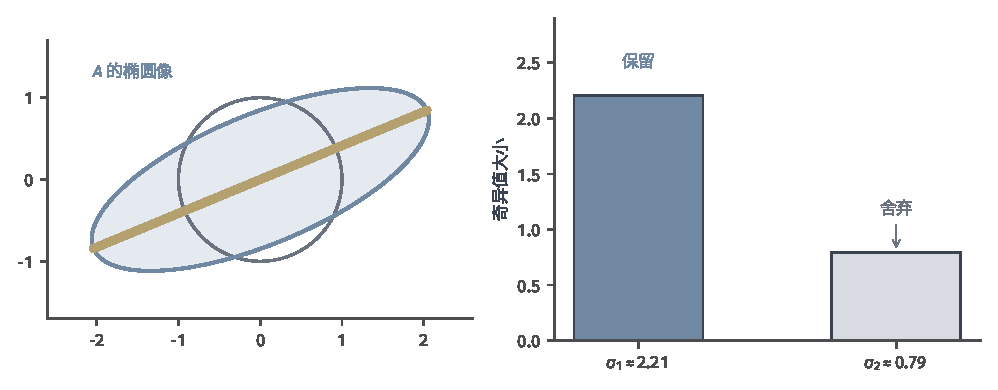
\includegraphics[width=168.998mm]{figures/00-shared/mathematical-preliminaries-upper/02-linear-spaces/matplotlib/ls-low-rank-truncation/ls-low-rank-truncation.pdf}
  \caption{低秩截断的几何。$\bm A=\left[\begin{smallmatrix}2&0.5\\0.5&1\end{smallmatrix}\right]$，
  灰圆为单位圆，蓝椭圆为$\bm A$的像。左：黄粗线段为秩一近似$\bm A_1=\sigma_1\bm v_1\bm v_1^\top$
  的像，椭圆被压成长$2\sigma_1$的线段；右：$\sigma_1\approx2.21$（保留）、$\sigma_2\approx0.79$
  （舍弃），算子范数误差$\lVert\bm A-\bm A_1\rVert_2=\sigma_2$。$\sigma_{1,2}=(3\pm\sqrt2)/2$。
  固定复算。}
  \label{fig:ls-low-rank-truncation}
\end{figure*}

\subsubsection{算法分析}

\paragraph{表示与计算代价}
截断SVD的好处在于表示代价。直接存储$\bm A$需要$md$个数；保存因子$\bm U_k$、$\sigma_1,\ldots,\sigma_k$与$\bm V_k$只需
\[
 k(m+d+1)
\]
个数。用$\bm A_k$乘向量时按
\[
 \bm A_k\bm x=\bm U_k\bigl(\bm\Sigma_k(\bm V_k^\top\bm x)\bigr)
\]
的顺序计算，依次需要约$dk$、$k$、$mk$次乘法，共$O(k(m+d))$次运算，而直接用$\bm A$乘向量需要$O(md)$次。

例如$m=d=1000$、$k=10$时，存储由$10^6$个数降为$20010$个数。形成完整的$\bm A_k=\bm U_k\bm W$约需$mdk$次乘法，只在需要矩阵本身或核验残差时才做。

这些是表示与后续作用的代价，不包括计算SVD本身的代价；后者取决于所用的数值算法，本书不作分析。

\paragraph{用途的区别}
第~\ref{chap:solution-error-regularization}章的截断SVD求解也用到$\bm A_k$，但那里是用它的伪逆稳定地求解方程；这里$\bm A_k$本身就是要评价的近似对象，评价标准是重建误差。$\bm A_k$的误差有多大、它在全部秩不超过$k$的矩阵中是否最好，由下一小节回答。

\subsection{最佳误差与最优性}
\label{sec:ls-truncated-svd-optimality}

\paragraph{截断SVD的误差}
截断SVD舍弃了后$r-k$项，误差应当由舍弃的奇异值决定。先把它算出来。设$0\leq k<r$，余下的部分是
\[
 \bm A-\bm A_k=\sum_{i=k+1}^r\sigma_i\bm u_i\bm v_i^\top .
\]
它仍由两组标准正交向量和降序的正系数$\sigma_{k+1}\geq\cdots\geq\sigma_r$组成，可以照第~\ref{sec:ls-svd-matrix-size}节的方法读出它的大小。

先看谱范数。把输入写成$\bm x=\sum_{i=1}^dc_i\bm v_i$，则
\[
 (\bm A-\bm A_k)\bm x=\sum_{i=k+1}^r\sigma_ic_i\bm u_i .
\]
由$\bm u_i$标准正交，
\[
 \lVert(\bm A-\bm A_k)\bm x\rVert_2^2=\sum_{i=k+1}^r\sigma_i^2c_i^2\leq\sigma_{k+1}^2\lVert\bm x\rVert_2^2,
\]
等号在$\bm x=\bm v_{k+1}$时成立。

再看Frobenius范数。由$\bm u_i^\top\bm u_j=\delta_{i,j}$，
\[
 (\bm A-\bm A_k)^\top(\bm A-\bm A_k)=\sum_{i=k+1}^r\sigma_i^2\bm v_i\bm v_i^\top ,
\]
取迹得Frobenius范数平方$\sum_{i>k}\sigma_i^2$。于是
\begin{equation}
\begin{gathered}
\lVert\bm A-\bm A_k\rVert_2=\sigma_{k+1}\\
\lVert\bm A-\bm A_k\rVert_{\mathrm F}
 =\Bigl(\sum_{i=k+1}^r\sigma_i^2\Bigr)^{1/2}.
\end{gathered}
\label{eq:ls-truncated-errors}
\end{equation}
Frobenius平方误差也可以由引理~\ref{lem:ls-low-rank-projection-error}读出：
\[
 \lVert\bm A\rVert_{\mathrm F}^2-\operatorname{tr}(\bm U_k^\top\bm A\bm A^\top\bm U_k)=\sum_{i\leq r}\sigma_i^2-\sum_{i\leq k}\sigma_i^2 .
\]
示例~\ref{ex:matrix-approximation-truncated-three-by-three}中$k=1$时，式~\eqref{eq:ls-truncated-errors}给出$\sqrt{1^2+1^2}=\sqrt2$与$\sigma_2=1$，与直接计算的$\bm E_1$一致。

\begin{example}[对角矩阵的截断误差]
\label{ex:ls-truncated-svd-diagonal}
取示例~\ref{ex:ls-low-rank-three-columns}中的$\bm A=\operatorname{diag}(3,2,1)$，奇异值为$3,2,1$，可取$\bm u_i=\bm v_i=\bm e_i$。截断得
\[
 \bm A_1=\operatorname{diag}(3,0,0),\qquad\bm A_2=\operatorname{diag}(3,2,0),
\]
残差为
\[
 \bm A-\bm A_1=\operatorname{diag}(0,2,1),\qquad\bm A-\bm A_2=\operatorname{diag}(0,0,1).
\]
$k=1$时平方误差$2^2+1^2=5$，谱范数误差$2$；$k=2$时平方误差与谱范数误差都是$1$。两者都与式~\eqref{eq:ls-truncated-errors}一致：
\[
 5=\sigma_2^2+\sigma_3^2,\qquad 2=\sigma_2,\qquad 1=\sigma_3 .
\]

平方误差$5$是只保留坐标直线$\bm e_1$时的损失，平方误差$1$是最佳坐标平面$\operatorname{span}\{\bm e_1,\bm e_2\}$的损失。
\end{example}

\paragraph{为什么还要比较全部候选}
两种误差记录的内容不同：Frobenius平方误差汇总所有舍弃方向，谱范数误差只记录最坏的单位输入方向。式~\eqref{eq:ls-truncated-errors}只是这一构造的误差，尚需证明其他秩不超过$k$的矩阵不能更小。

Frobenius范数的结论由上一小节的化归和迹极值得到。谱范数不能这样处理，因为
\[
 \lVert\bm M\rVert_2\leq\lVert\bm M\rVert_{\mathrm F},
\]
Frobenius误差的下界推不出谱范数误差的下界，需要另作证明。

谱范数下界的想法是：秩不超过$k$的$\bm X$至少把一个$(d-k)$维子空间送到零，这个子空间一定与前$k+1$个右奇异方向相交；在交点处，$\bm A-\bm X$的作用就是$\bm A$本身的作用，而$\bm A$在前$k+1$个方向上至少放大$\sigma_{k+1}$倍。

下面用一个例子说明这一想法。取$\bm A=\operatorname{diag}(3,2,1)$、$k=1$，并取一个不同于截断SVD的秩一候选：
\[
 \bm X=\begin{bmatrix}3&2&0\\0&0&0\\0&0&0\end{bmatrix}.
\]
它的核是$\{\bm x:3x_1+2x_2=0\}$，与$\operatorname{span}\{\bm e_1,\bm e_2\}$交于
\[
 \bm x=\frac1{\sqrt{13}}\begin{bmatrix}2\\-3\\0\end{bmatrix}.
\]
在这个单位向量上$\bm X\bm x=\bm0$，于是
\[
 (\bm A-\bm X)\bm x=\bm A\bm x=\frac1{\sqrt{13}}\begin{bmatrix}6\\-6\\0\end{bmatrix},
\]
它的长度为
\[
 \lVert\bm A\bm x\rVert_2=\sqrt{72/13}\approx2.353\geq\sigma_2=2 .
\]
所以这个候选的谱范数误差至少为$2.353$，不比截断SVD好。下面的定理对任意候选作同样的论证。

\begin{theorem}[Eckart--Young--Mirsky最佳低秩逼近]
\label{thm:ls-best-low-rank}
\label{thm:matrix-analysis-best-low-rank}
设$\bm A\in\mathbb R^{m\times d}$的秩为$r$，奇异值为$\sigma_1\geq\cdots\geq\sigma_r>0$。对$0\leq k<r$，
\begin{align}
 \min_{\operatorname{rank}\bm X\leq k}\lVert\bm A-\bm X\rVert_2
 &=\sigma_{k+1},
 \label{eq:matrix-analysis-best-rank-k-spectral}\\
 \min_{\operatorname{rank}\bm X\leq k}\lVert\bm A-\bm X\rVert_{\mathrm F}
 &=\Bigl(\sum_{i=k+1}^r\sigma_i^2\Bigr)^{1/2},
 \label{eq:matrix-analysis-best-rank-k-frobenius}
\end{align}
两个最小值都由截断SVD$\bm A_k$达到。
\end{theorem}
\begin{proof}
由式~\eqref{eq:ls-truncated-errors}，$\bm A_k$的两种误差恰为右端，只需证明任意秩不超过$k$的$\bm X$误差都不更小。$k=0$时只有$\bm X=\bm0$，结论即式~\eqref{eq:ls-truncated-errors}，下设$k\geq1$。

Frobenius情形。按第~\ref{sec:ls-low-rank-projection-error}节的做法，把$\bm X$的列空间补成一个$k$维子空间，取其标准正交基组成$\bm Y$，则$\bm X=\bm Y\bm C$。由引理~\ref{lem:ls-low-rank-projection-error}、定理~\ref{thm:matrix-analysis-trace-minimum}与式~\eqref{eq:matrix-analysis-frobenius-norm}，
\[
 \begin{aligned}
 \lVert\bm A-\bm X\rVert_{\mathrm F}^2
 &\geq\lVert\bm A\rVert_{\mathrm F}^2-\operatorname{tr}(\bm Y^\top\bm A\bm A^\top\bm Y)\\
 &\geq\sum_{i=1}^r\sigma_i^2-\sum_{i=1}^k\sigma_i^2=\sum_{i=k+1}^r\sigma_i^2 .
 \end{aligned}
\]

谱范数情形。由秩零度定理~\ref{thm:ls-rank-nullity}，
\[
 \dim\ker\bm X=d-\operatorname{rank}\bm X\geq d-k .
\]
子空间$\operatorname{span}\{\bm v_1,\ldots,\bm v_{k+1}\}$的维数为$k+1$（$k+1\leq r\leq d$）。两者维数之和超过$d$，由维数公式，它们有非零公共向量；取其中的单位向量$\bm x=\sum_{i=1}^{k+1}c_i\bm v_i$，$\sum_ic_i^2=1$。由$\bm X\bm x=\bm0$，
\begin{equation}
 \lVert(\bm A-\bm X)\bm x\rVert_2
 =\lVert\bm A\bm x\rVert_2
 =\Bigl(\sum_{i=1}^{k+1}\sigma_i^2c_i^2\Bigr)^{1/2}
 \geq\sigma_{k+1},
 \label{eq:ls-spectral-lower-bound}
\end{equation}
所以$\lVert\bm A-\bm X\rVert_2\geq\sigma_{k+1}$。
\end{proof}

在上面的秩一候选中，$c_1=2/\sqrt{13}$、$c_2=-3/\sqrt{13}$，式~\eqref{eq:ls-spectral-lower-bound}的中间量为
\[
 \sigma_1^2c_1^2+\sigma_2^2c_2^2=9\cdot\frac4{13}+4\cdot\frac9{13}=\frac{72}{13}\geq\sigma_2^2=4 ,
\]
与直接计算一致。

这一结论最早由Eckart与Young给出\scite{eckart1936}。定理覆盖任意秩不超过$k$的矩阵，而不只覆盖事先选定的投影形式：Frobenius情形借助第~\ref{sec:ls-low-rank-projection-error}节的化归把任意候选归入某个子空间，谱范数情形则直接利用候选矩阵的核。两种范数下的最小误差都由舍弃的奇异值决定：谱范数看最大的舍弃值$\sigma_{k+1}$，Frobenius范数看全部舍弃值的平方和。

\subsection{最优解的唯一性}
\label{sec:matrix-approximation-low-rank-uniqueness}

\paragraph{Frobenius情形}
最小误差唯一，达到最小误差的矩阵却未必唯一。示例~\ref{ex:matrix-approximation-truncated-three-by-three}中的$\bm A_2$与$\bm A_2'$已经说明了这一点。问题是：什么条件下最优矩阵只有一个？在有效的秩预算$1\leq k<r$下，Frobenius情形的答案由迹极值的取等条件决定，关键是截断位置两侧的奇异值是否有间隙。

\begin{theorem}[Frobenius最佳逼近的唯一性]
\label{thm:ls-best-low-rank-uniqueness}
设$1\leq k<r$且$\sigma_k>\sigma_{k+1}$，则$\bm A_k$是$\min_{\operatorname{rank}\bm X\leq k}\lVert\bm A-\bm X\rVert_{\mathrm F}$的唯一最优解。
\end{theorem}
\begin{proof}
设$\bm X$达到最小值，按定理~\ref{thm:ls-best-low-rank}的证明取$\bm Y$，写$\bm X=\bm Y\bm C$。证明中的两个不等号都须取等。第一个取等，由式~\eqref{eq:ls-low-rank-projection-split}得$\bm C=\bm Y^\top\bm A$，即
\[
 \bm X=\bm Y\bm Y^\top\bm A .
\]

第二个取等，即
\[
 \operatorname{tr}(\bm Y^\top\bm A\bm A^\top\bm Y)=\sum_{i=1}^k\sigma_i^2 .
\]
$\bm A\bm A^\top$的第$k$与第$k+1$个特征值为$\sigma_k^2>\sigma_{k+1}^2$，由定理~\ref{thm:matrix-analysis-trace-minimum}的取等条件，$\operatorname{range}(\bm Y)=\operatorname{span}\{\bm u_1,\ldots,\bm u_k\}$。

到同一子空间的正交投影是同一个矩阵，故$\bm Y\bm Y^\top=\bm U_k\bm U_k^\top$，从而
\[
 \bm X=\bm U_k\bm U_k^\top\bm A=\bm A_k .
\]
\end{proof}

$k=1$时，条件$\sigma_1>\sigma_2$正是第~\ref{sec:matrix-approximation-rank-one-solution}节秩一最优解唯一的条件。

间隙条件也确定了$\bm A_k$本身：$\sigma_k>\sigma_{k+1}$时，$\operatorname{span}\{\bm u_1,\ldots,\bm u_k\}$是$\bm A\bm A^\top$前$k$个特征值对应的特征空间之和，不随SVD的选取改变，$\bm A_k=\bm U_k\bm U_k^\top\bm A$也就与所选的奇异向量无关。示例~\ref{ex:matrix-approximation-truncated-three-by-three}中$k=1$时$\sigma_1=5>\sigma_2=1$，$\bm A_1$唯一；$k=2$时$\sigma_2=\sigma_3$，定理不适用。

截断跨过相等的正奇异值时，唯一性失败。例如$\bm A=\operatorname{diag}(2,1,1)$、$k=2$，下面两个矩阵都是最优解：
\[
 \operatorname{diag}(2,1,0),\qquad\operatorname{diag}(2,0,1).
\]
它们的残差分别是$\operatorname{diag}(0,0,1)$与$\operatorname{diag}(0,1,0)$，平方误差都是$1=\sigma_3^2$。这时“前$k$个奇异向量”本身就有不同选法，每种选法给出一个最优矩阵；三阶例中的$\bm A_2$与$\bm A_2'$也是这种情形。

\paragraph{谱范数情形}
谱范数下的最优矩阵即使有间隙也不唯一，所以间隙条件不能直接当成谱范数的唯一性保证。先说明对角矩阵的谱范数。$\bm D=\operatorname{diag}(a_1,\ldots,a_m)$满足
\[
 \lVert\bm D\bm x\rVert_2^2=\sum_ia_i^2x_i^2\leq\max_ia_i^2\,\lVert\bm x\rVert_2^2 ,
\]
在绝对值最大的对角元所在的坐标向量处取等，故
\[
 \lVert\bm D\rVert_2=\max_i\lvert a_i\rvert .
\]
取$\bm A=\operatorname{diag}(3,2,1)$、$k=1$，候选$\bm X=\operatorname{diag}(t,0,0)$给出残差$\operatorname{diag}(3-t,2,1)$，于是
\[
 \lVert\bm A-\bm X\rVert_2=\max(\lvert3-t\rvert,2).
\]
$1\leq t\leq5$时它都等于最小值$2$，尽管$\sigma_1=3>\sigma_2=2$。例如$t=2$时残差是$\operatorname{diag}(1,2,1)$，最坏方向仍是$\bm e_2$。谱范数只看最坏方向，最坏方向之外的偏差在一定范围内可以随意改变。

Frobenius范数则不同：同一族候选的平方误差是
\[
 \lVert\bm A-\bm X\rVert_{\mathrm F}^2=(3-t)^2+5 ,
\]
只在$t=3$时取到最小值$5$。

\paragraph{边界情形与适用范围}
边界情形$k=0$与$k\geq r$已在第~\ref{sec:matrix-approximation-problem}节回答，最优矩阵分别是$\bm0$与$\bm A$本身，不需要套用间隙判据。

本节的最优性依赖两个前提：允许集合是全部秩不超过$k$的矩阵，误差是谱范数或Frobenius范数。额外要求近似矩阵非负或因子稀疏时，允许集合缩小，$\bm A_k$可能不再可行。改用逐元素加权的平方误差
\[
 \sum_{i,j}w_{i,j}(a_{i,j}-x_{i,j})^2
\]
时，误差一般不再按正交投影分解，引理~\ref{lem:ls-low-rank-projection-error}失效。这些情形下截断SVD一般不再是最优解，最优性需要重新论证；下一节处理其中能够化归的一类加权误差。

% 第15章第4节：加权逼近与广义Rayleigh商（广义Rayleigh商的极值、加权低秩逼近）。

\section{加权逼近与广义Rayleigh商}
\label{sec:ls-generalized-rayleigh}

前两节都用欧氏长度：单位方向按$\bm u^\top\bm u=1$规定，重建误差按各元素平方和计算。各坐标的单位或重要性不同时，长度往往按第~\ref{chap:inner-product-spaces}章的加权内积度量。度量一变，有两处跟着改变：规定“单位方向”的长度变了，比较重建误差的标准也变了。

本节先处理前一处：保持二次型不变，改用加权长度规定单位方向，得到广义Rayleigh商及其极值。再处理后一处：在行、列权重可以分离的误差下研究低秩逼近，并看到它的最佳方向正是由广义Rayleigh商选出的。广义Rayleigh商还为后面的图谱松弛提供工具：卷九的谱划分把平衡约束写成按顶点度加权的长度，再用广义Rayleigh商的极值给出离散划分问题的松弛下界，可参考\BookChapterRef{chap:spectral-partition}{卷九“谱划分”章}。

\subsection{广义Rayleigh商的极值}
\label{sec:ls-generalized-eigen-reduction}
\label{sec:ls-generalized-eigen-check}

保持$\bm S=\operatorname{diag}(4,1)$不变，改用$\bm B=\operatorname{diag}(9,1)$规定长度，即要求
\[
 \bm x^\top\bm B\bm x=9x_1^2+x_2^2=1 .
\]
沿第一坐标方向，满足约束的向量是$\pm\bm e_1/3$；沿第二坐标方向，满足约束的向量仍是$\pm\bm e_2$。两者的二次型值分别为
\[
 \Bigl(\frac{\bm e_1}3\Bigr)^{\!\top}\bm S\,\frac{\bm e_1}3=4\cdot\Bigl(\frac13\Bigr)^2=\frac49,\qquad
 \bm e_2^\top\bm S\bm e_2=1 .
\]
在欧氏约束下最优的$\bm e_1$方向，现在不如$\bm e_2$方向。

可见改变长度标准会改变答案。而且与示例~\ref{ex:ls-rayleigh-diagonal-two-by-two}之前的讨论一样，比较两个坐标方向还不够，必须比较全部满足加权约束的方向。与欧氏情形相同，先把约束化为一个不随缩放改变的商。
\begin{definition}[广义Rayleigh商]
\label{def:ls-generalized-rayleigh-quotient}
设$\bm S\in\mathbb R^{d\times d}$对称，$\bm B\in\mathbb R^{d\times d}$对称正定。对$\bm x\neq\bm0$，称
\begin{equation}
 R_{\bm S,\bm B}(\bm x)=\frac{\bm x^\top\bm S\bm x}{\bm x^\top\bm B\bm x}
 \label{eq:ls-generalized-rayleigh-quotient}
\end{equation}
为$\bm S$关于$\bm B$的\term{广义Rayleigh商}（generalized Rayleigh quotient）。
\end{definition}
$\bm B$正定保证分母$\bm x^\top\bm B\bm x$对一切$\bm x\neq\bm0$为正，商有定义。把$\bm x$换成$c\bm x$（$c\neq0$）时分子分母同乘$c^2$，商不变。

对任意$\bm x\neq\bm0$，令$\bm u=\bm x/\sqrt{\bm x^\top\bm B\bm x}$，则
\[
 \bm u^\top\bm B\bm u=1,\qquad R_{\bm S,\bm B}(\bm x)=\bm u^\top\bm S\bm u ;
\]
反过来，约束$\bm x^\top\bm B\bm x=1$上的二次型值就是广义Rayleigh商。所以求广义Rayleigh商的极值，等价于在$\bm x^\top\bm B\bm x=1$上比较$\bm x^\top\bm S\bm x$。

$\bm B=\bm I$时，广义Rayleigh商恰好回到普通Rayleigh商。两者比较的是同一个二次型$\bm x^\top\bm S\bm x$，差别只在于用哪种长度规定“单位输入”：普通Rayleigh商用欧氏长度，广义Rayleigh商用加权长度$\lVert\bm x\rVert_{\bm B}$。

\subsubsection{主要思想}

\paragraph{把加权长度换成欧氏长度}
加权约束$\bm x^\top\bm B\bm x=1$的困难在于它不是欧氏单位球面，第~\ref{sec:ls-rayleigh-extremal}节的结论不能直接使用。思路是换一个坐标，使加权长度在新坐标中成为欧氏长度。

先看开头的例子。约束可以改写成两个平方之和：
\[
 9x_1^2+x_2^2=(3x_1)^2+x_2^2 .
\]
令$z_1=3x_1$、$z_2=x_2$，约束就成为欧氏单位圆$z_1^2+z_2^2=1$。二次型也用新坐标表示，由$x_1=z_1/3$得
\[
 4x_1^2+x_2^2=\frac49z_1^2+z_2^2 .
\]
于是加权约束下的问题，变成了对角矩阵$\operatorname{diag}(4/9,1)$在欧氏单位圆上的普通Rayleigh商问题。

一般的$\bm B$不是对角矩阵，但同样可以写成平方和。设$\bm L$是上三角矩阵，令$\bm z=\bm L\bm x$。二阶时按元素写出
\[
 \begin{bmatrix}z_1\\z_2\end{bmatrix}
 =\begin{bmatrix}l_{1,1}&l_{1,2}\\0&l_{2,2}\end{bmatrix}
 \begin{bmatrix}x_1\\x_2\end{bmatrix}
 =\begin{bmatrix}l_{1,1}x_1+l_{1,2}x_2\\l_{2,2}x_2\end{bmatrix},
\]
展开平方和得
\[
 \begin{aligned}
 z_1^2+z_2^2
 &=l_{1,1}^2x_1^2+2l_{1,1}l_{1,2}x_1x_2+(l_{1,2}^2+l_{2,2}^2)x_2^2\\
 &=\bm x^\top
 \begin{bmatrix}l_{1,1}^2&l_{1,1}l_{1,2}\\l_{1,1}l_{1,2}&l_{1,2}^2+l_{2,2}^2\end{bmatrix}
 \bm x .
 \end{aligned}
\]
中间的矩阵正是$\bm L^\top\bm L$。所以只要$\bm B=\bm L^\top\bm L$，加权长度$\bm x^\top\bm B\bm x$在新坐标中就是欧氏长度$\bm z^\top\bm z$。开头的例子对应$\bm L=\operatorname{diag}(3,1)$。

这样的$\bm L$总是存在。由定理~\ref{thm:ls-gram-factor}，正定的$\bm B$可以写成$\bm B=\bm L^\top\bm L$，其中$\bm L$可逆。于是$\bm x=\bm L^{-1}\bm z$，且$\bm x\neq\bm0$当且仅当$\bm z\neq\bm0$。

\paragraph{化为普通Rayleigh商}
把$\bm x=\bm L^{-1}\bm z$代入分子与分母，得
\[
 \bm x^\top\bm B\bm x=(\bm L\bm x)^\top(\bm L\bm x)=\bm z^\top\bm z,\qquad
 \bm x^\top\bm S\bm x=\bm z^\top\bm L^{-\top}\bm S\bm L^{-1}\bm z ,
\]
其中$\bm L^{-\top}$表示$(\bm L^{-1})^\top$。记
\begin{equation}
 \bm C=\bm L^{-\top}\bm S\bm L^{-1}.
 \label{eq:ls-generalized-rayleigh-reduced-matrix}
\end{equation}
由$\bm S$对称，
\[
 \bm C^\top=\bm L^{-\top}\bm S^\top\bm L^{-1}=\bm C ,
\]
所以$\bm C$仍是实对称矩阵。广义Rayleigh商在新坐标中写成
\begin{equation}
 R_{\bm S,\bm B}(\bm x)=\frac{\bm z^\top\bm C\bm z}{\bm z^\top\bm z}=R_{\bm C}(\bm L\bm x).
 \label{eq:ls-generalized-rayleigh-reduction}
\end{equation}
加权约束问题就化成了$\bm C$的普通Rayleigh商问题，可以直接应用定理~\ref{thm:matrix-analysis-rayleigh-ritz}。

这一化归只用到Gram因子与换元，不需要矩阵平方根、多元微分或Lagrange乘子法。开头的例子中$\bm C=\operatorname{diag}(4/9,1)$，正是上面按元素得到的矩阵。

\paragraph{换回原坐标}
$\bm C$的最优方向在新坐标中，还要换回原坐标。若$\bm C\bm z=\mu\bm z$，令$\bm v=\bm L^{-1}\bm z$，则
\[
 \bm L^{-\top}\bm S\bm v=\mu\bm L\bm v .
\]
两边左乘$\bm L^\top$，得
\[
 \bm S\bm v=\mu\bm L^\top\bm L\bm v=\mu\bm B\bm v .
\]
反过来，若$\bm S\bm v=\mu\bm B\bm v$且$\bm v\neq\bm0$，左乘$\bm L^{-\top}$并令$\bm z=\bm L\bm v$，就得到$\bm C\bm z=\mu\bm z$。所以，$\bm C$的特征对与下面方程的解一一对应。

\begin{definition}[广义特征值]
\label{def:matrix-analysis-generalized-eigenvalue}
对实对称$\bm S$与对称正定$\bm B$，称满足
\begin{equation}
\begin{gathered}
\bm S\bm v=\mu\bm B\bm v\\
\bm v\neq\bm0
\end{gathered}
\label{eq:matrix-analysis-generalized-eigenproblem}
\end{equation}
的$\mu$为广义特征值，$\bm v$为属于$\mu$的广义特征向量，求解它们的问题称为\term{广义特征问题}（generalized eigenvalue problem）。
\end{definition}

广义特征值不依赖Gram因子$\bm L$的选取。由$\bm S-\mu\bm B=\bm L^\top(\bm C-\mu\bm I)\bm L$，
\[
 \det(\bm S-\mu\bm B)=(\det\bm L)^2\det(\bm C-\mu\bm I),
\]
而$\det\bm L\neq0$，所以广义特征值恰是$\det(\bm S-\mu\bm B)=0$的根，也就是$\bm C$的特征值。不同的$\bm L$给出不同的$\bm C$，特征值却相同。

$\bm C$对称，由谱定理，这些根全是实数，按重数计共有$d$个，下面记为$\mu_1\geq\cdots\geq\mu_d$。

\paragraph{极值与最优方向}
把定理~\ref{thm:matrix-analysis-rayleigh-ritz}用于$\bm C$并换回原坐标，就得到加权约束问题的解。

\begin{theorem}[广义Rayleigh商的极值]
\label{thm:ls-generalized-rayleigh-extremal}
设$\bm S$对称、$\bm B$对称正定，广义特征值为$\mu_1\geq\cdots\geq\mu_d$。则对一切$\bm x\neq\bm0$，
\begin{equation}
 \mu_d\leq R_{\bm S,\bm B}(\bm x)\leq\mu_1 .
 \label{eq:ls-generalized-rayleigh-extremal}
\end{equation}
$R_{\bm S,\bm B}(\bm x)=\mu_1$当且仅当$\bm S\bm x=\mu_1\bm B\bm x$，$R_{\bm S,\bm B}(\bm x)=\mu_d$当且仅当$\bm S\bm x=\mu_d\bm B\bm x$。因此，在约束$\bm x^\top\bm B\bm x=1$上，$\bm x^\top\bm S\bm x$的最大值为$\mu_1$，最优解是满足$\bm v^\top\bm B\bm v=1$的属于$\mu_1$的广义特征向量；最小值的情形相同。
\end{theorem}
\begin{proof}
取$\bm B=\bm L^\top\bm L$与$\bm C=\bm L^{-\top}\bm S\bm L^{-1}$如上。$\bm C$的特征值就是$\mu_1\geq\cdots\geq\mu_d$。对$\bm x\neq\bm0$，令$\bm z=\bm L\bm x\neq\bm0$，由$R_{\bm S,\bm B}(\bm x)=R_{\bm C}(\bm z)$及定理~\ref{thm:matrix-analysis-rayleigh-ritz}，得$\mu_d\leq R_{\bm S,\bm B}(\bm x)\leq\mu_1$。

同一定理还说明，$R_{\bm C}(\bm z)=\mu_1$当且仅当$\bm C\bm z=\mu_1\bm z$。由上面的一一对应，这又当且仅当$\bm S\bm x=\mu_1\bm B\bm x$。$\bm C$确有属于$\mu_1$的特征向量，所以上界能够取到。最小值同理。

最后，约束$\bm x^\top\bm B\bm x=1$上的二次型值就是广义Rayleigh商，所以它的最大值为$\mu_1$，且只在满足$\bm S\bm x=\mu_1\bm B\bm x$与$\bm x^\top\bm B\bm x=1$的$\bm x$处取到。
\end{proof}

\paragraph{\texorpdfstring{$\bm B$}{B}正交的广义特征向量}
上面只用到$\bm C$两端的特征向量。对$\bm C$应用完整的谱分解，还能得到全部广义特征向量的结构：它们可以选得关于加权内积$\langle\cdot,\cdot\rangle_{\bm B}$互相正交。

\begin{theorem}[$\bm B$正交的广义特征向量]
\label{thm:ls-generalized-eigen-b-orthogonal}
设$\bm S$对称、$\bm B$对称正定，广义特征值为$\mu_1\geq\cdots\geq\mu_d$。则存在$\bm v_1,\ldots,\bm v_d$，使
\begin{equation}
 \bm S\bm v_i=\mu_i\bm B\bm v_i,\qquad \bm v_i^\top\bm B\bm v_j=\delta_{i,j}\quad(i,j=1,\ldots,d).
 \label{eq:ls-generalized-eigen-b-orthogonal}
\end{equation}
记$\bm V=[\bm v_1,\ldots,\bm v_d]$，$\bm M=\operatorname{diag}(\mu_1,\ldots,\mu_d)$，上式等价于$\bm V^\top\bm B\bm V=\bm I$与$\bm V^\top\bm S\bm V=\bm M$。
\end{theorem}
\begin{proof}
由谱定理，$\bm C=\bm Z\bm M\bm Z^\top$，其中$\bm Z=[\bm z_1,\ldots,\bm z_d]$为正交矩阵，$\bm C\bm z_i=\mu_i\bm z_i$。令$\bm V=\bm L^{-1}\bm Z$，即$\bm v_i=\bm L^{-1}\bm z_i$。由上面的一一对应，$\bm S\bm v_i=\mu_i\bm B\bm v_i$。又
\[
\begin{gathered}
 \bm V^\top\bm B\bm V=\bm Z^\top\bm L^{-\top}\bm L^\top\bm L\bm L^{-1}\bm Z=\bm Z^\top\bm Z=\bm I,\\
 \bm V^\top\bm S\bm V=\bm Z^\top\bm L^{-\top}\bm S\bm L^{-1}\bm Z=\bm Z^\top\bm C\bm Z=\bm M .
\end{gathered}
\]
逐元素比较第一式即得$\bm v_i^\top\bm B\bm v_j=\delta_{i,j}$。
\end{proof}

$\bm V$可逆，所以任意$\bm x$都能写成$\bm x=\sum_ia_i\bm v_i$。由定理，
\[
 \bm x^\top\bm B\bm x=\sum_{i=1}^da_i^2,\qquad \bm x^\top\bm S\bm x=\sum_{i=1}^d\mu_ia_i^2 .
\]
广义Rayleigh商再次成为特征值的加权平均。这与普通情形完全平行，只是坐标改成了$\bm B$正交的广义特征向量。

至此两端极值都已求出。若还需要刻画中间的广义特征值，可以对$\bm C$使用第~\ref{sec:ls-spectral-value-sensitivity}节的Courant--Fischer最小最大原理（定理~\ref{thm:matrix-analysis-courant-fischer}），再按$\bm z=\bm L\bm x$换回原坐标。

\paragraph{用开头的例子核对}
最后回到开头的二维例子，把上面的结论逐一落实，并与直接比较全部可行方向的结果对照。

\begin{example}[加权约束下的最优方向]
\label{ex:ls-generalized-rayleigh-diagonal}
取$\bm S=\operatorname{diag}(4,1)$与$\bm B=\operatorname{diag}(9,1)$，在加权约束$\bm x^\top\bm B\bm x=1$下求$\bm x^\top\bm S\bm x$的最大值、最小值与最优方向。

由$\bm L=\operatorname{diag}(3,1)$得$\bm C=\operatorname{diag}(4/9,1)$。由定理~\ref{thm:matrix-analysis-rayleigh-ritz}，$R_{\bm C}$的最大值为$1$，在$\bm z=\pm\bm e_2$取到；最小值为$4/9$，在$\bm z=\pm\bm e_1$取到。换回原坐标$\bm v=\bm L^{-1}\bm z$，得到
\[
 \text{最大方向}\ \pm\bm e_2,\qquad \text{最小方向}\ \pm\frac{\bm e_1}{3}.
\]

两者都满足加权单位约束：
\[
 \bm e_2^\top\bm B\bm e_2=1,\qquad \Bigl(\frac{\bm e_1}{3}\Bigr)^{\!\top}\bm B\,\frac{\bm e_1}{3}=\frac99=1 .
\]
它们也满足广义特征方程：
\[
 \bm S\bm e_2=\bm e_2=1\cdot\bm B\bm e_2,\qquad
 \bm S\frac{\bm e_1}{3}=\frac43\bm e_1=\frac49\cdot\bm B\frac{\bm e_1}{3},
\]
分别属于$1$与$4/9$；又$\bm e_2^\top\bm B(\bm e_1/3)=0$，满足$\bm B$正交。

不经化归，也可以直接比较全部可行方向。约束给出$x_2^2=1-9x_1^2$，其中$x_1^2\in[0,1/9]$，于是
\[
 \bm x^\top\bm S\bm x=4x_1^2+1-9x_1^2=1-5x_1^2\in\Bigl[\frac49,1\Bigr].
\]
最大值$1$在$x_1=0$即$\pm\bm e_2$处取到，最小值$4/9$在$x_1^2=1/9$即$\pm\bm e_1/3$处取到，与化归的结果一致。

对照示例~\ref{ex:ls-rayleigh-diagonal-two-by-two}：同一个$\bm S$在欧氏约束下的最大方向是$\bm e_1$。加权约束让沿$\bm e_1$的可行向量缩短为$\bm e_1/3$，最大方向就换成了$\bm e_2$。
\end{example}

\subsubsection{算法实现}

上面的例子中$\bm L$是对角矩阵，可以直接求逆。一般情形下，计算也按化归的顺序进行：先求Gram因子，再形成$\bm C$，对$\bm C$作谱分解，最后换回原坐标；换元通过因子分解与三角求解完成，不必显式形成$\bm L^{-1}$。输入是对称的$\bm S$与对称正定的$\bm B$，输出是所需的广义特征值与满足$\bm v^\top\bm B\bm v=1$的广义特征向量。下面用以下新的二维示例逐步演示。

\begin{example}[按三角求解的步骤计算]
\label{ex:matrix-approximation-generalized-cholesky}
取
\[
 \bm S=\begin{bmatrix}2&0\\0&3\end{bmatrix},\qquad
 \bm B=\begin{bmatrix}4&0\\0&1\end{bmatrix},
\]
在约束$\bm x^\top\bm B\bm x=1$下求$\bm x^\top\bm S\bm x$的最大值、最小值与最优方向。
\end{example}

\paragraph{变量}
\begin{itemize}
 \item $\bm L\in\mathbb R^{d\times d}$：$\bm B$的上三角Gram因子，满足$\bm B=\bm L^\top\bm L$。
 \item $\bm W\in\mathbb R^{d\times d}$：中间矩阵$\bm W=\bm L^{-\top}\bm S$。
 \item $\bm C\in\mathbb R^{d\times d}$：化归后的对称矩阵$\bm C=\bm W\bm L^{-1}$。
 \item $\mu_i$与$\bm z_i$：$\bm C$的特征值与单位特征向量，$\mu_i$按降序排列。
 \item $\bm v_i$：换回原坐标后的广义特征向量。
\end{itemize}

\paragraph{输入与预处理}
用第~\ref{sec:ls-cholesky}节的Cholesky分解求出$\bm B=\bm G\bm G^\top$，其中$\bm G$是对角元为正的下三角矩阵，再取
\[
 \bm L=\bm G^\top ,
\]
它是上三角矩阵，满足$\bm B=\bm L^\top\bm L$。若分解中某个开方量不为正，说明$\bm B$不是正定矩阵，正定化归不能继续使用，停止并报告。

例中$\bm B$是对角矩阵，Cholesky分解直接对对角元开方：
\[
 \bm L=\begin{bmatrix}2&0\\0&1\end{bmatrix}.
\]

\paragraph{计算步骤}
\begin{enumerate}
 \item \textbf{形成$\bm W$。}解三角方程组
 \begin{equation}
  \bm L^\top\bm W=\bm S .
  \label{eq:ls-generalized-solve-w}
 \end{equation}
 $\bm L^\top$是下三角矩阵，对$\bm S$的每一列按式~\eqref{eq:ls-forward-substitution}作前代。

 例中$\bm L^\top=\operatorname{diag}(2,1)$，每个方程只含一个未知元：$2w_{1,1}=2$，$w_{2,2}=3$，非对角元的方程右端为零。于是
 \[
  \bm W=\begin{bmatrix}1&0\\0&3\end{bmatrix}.
 \]

 \item \textbf{形成$\bm C$。}由$\bm C=\bm W\bm L^{-1}$得$\bm C\bm L=\bm W$，转置后成为
 \begin{equation}
  \bm L^\top\bm C^\top=\bm W^\top ,
  \label{eq:ls-generalized-solve-c}
 \end{equation}
 仍是以下三角矩阵为系数的方程组，再作一次前代。$\bm C$对称，解出的$\bm C^\top$就是$\bm C$；舍入误差会使算出的两半略有差别，通常取$(\bm C+\bm C^\top)/2$再进入下一步，以保持对称结构。

 例中$2c_{1,1}=1$，$c_{2,2}=3$，于是
 \[
  \bm C=\begin{bmatrix}1/2&0\\0&3\end{bmatrix}.
 \]

 \item \textbf{对$\bm C$作谱分解。}对对称矩阵$\bm C$作正交谱分解，按降序取出特征值与单位特征向量；只需要最大值或最小值时，只取相应的一对。例中
 \[
  \mu_1=3,\quad \bm z_1=\bm e_2;\qquad \mu_2=\frac12,\quad \bm z_2=\bm e_1 .
 \]

 \item \textbf{换回原坐标。}对每个所需的$\bm z_i$解三角方程组
 \begin{equation}
  \bm L\bm v_i=\bm z_i ,
  \label{eq:ls-generalized-recover-v}
 \end{equation}
 $\bm L$是上三角矩阵，按式~\eqref{eq:ls-back-substitution}作回代。由$\bm v_i^\top\bm B\bm v_i=\bm z_i^\top\bm z_i=1$，所得$\bm v_i$自动满足加权单位约束。

 例中$\bm L\bm v_1=\bm e_2$与$\bm L\bm v_2=\bm e_1$分别给出
 \[
  \bm v_1=\begin{bmatrix}0\\1\end{bmatrix},\qquad \bm v_2=\begin{bmatrix}1/2\\0\end{bmatrix}.
 \]

 \item \textbf{核验。}在原坐标中计算广义特征残差$\bm S\bm v_i-\mu_i\bm B\bm v_i$与加权长度$\bm v_i^\top\bm B\bm v_i$，确认前者接近零、后者接近$1$。例中
 \[
  \bm S\bm v_1=\begin{bmatrix}0\\3\end{bmatrix}=3\,\bm B\bm v_1,\qquad
  \bm S\bm v_2=\begin{bmatrix}1\\0\end{bmatrix}=\frac12\begin{bmatrix}2\\0\end{bmatrix}=\frac12\,\bm B\bm v_2 ,
 \]
 两个残差都为零。加权长度为
 \[
  \bm v_1^\top\bm B\bm v_1=1,\qquad \bm v_2^\top\bm B\bm v_2=\Bigl(\frac12\Bigr)^2\cdot4=1 .
 \]
\end{enumerate}

最终得到加权约束下的最大值、最小值与最优方向。例中
\[
 \begin{aligned}
 \max_{\bm x^\top\bm B\bm x=1}\bm x^\top\bm S\bm x&=3, &&\text{在}\ \pm\begin{bmatrix}0\\1\end{bmatrix}\ \text{取到};\\
 \min_{\bm x^\top\bm B\bm x=1}\bm x^\top\bm S\bm x&=\frac12, &&\text{在}\ \pm\begin{bmatrix}1/2\\0\end{bmatrix}\ \text{取到}.
 \end{aligned}
\]

与欧氏约束比较：$\bm S$的普通Rayleigh商最大为$3$、最小为$2$，最优直线同样是两条坐标轴。这里加权没有改变最优直线，却把最小值由$2$变成$1/2$，因为沿$\bm e_1$满足加权约束的向量缩短为$\bm e_1/2$。与示例~\ref{ex:ls-generalized-rayleigh-diagonal}合起来看，长度标准既可能改变最优方向，也可能只改变最优值。

\subsubsection{算法分析}

\paragraph{运算量}
形成$\bm C$只用到Cholesky分解与以三角矩阵为系数的求解，代价都是$O(d^3)$次运算；之后的主要代价在对称特征值计算，所用算法本书不作分析。只需要最大或最小的广义特征对时，也必须先完成同样的换元，因为$\bm S$本身的特征向量一般不是广义特征向量。

\paragraph{为什么不改求普通特征问题}
另一种看似直接的做法是把$\bm S\bm v=\mu\bm B\bm v$左乘$\bm B^{-1}$，改求普通特征问题
\[
 \bm B^{-1}\bm S\bm v=\mu\bm v .
\]
由$\bm B^{-1}=\bm L^{-1}\bm L^{-\top}$，
\[
 \bm B^{-1}\bm S=\bm L^{-1}\bm L^{-\top}\bm S=\bm L^{-1}\bm C\bm L ,
\]
它与$\bm C$相似，特征值相同；但$\bm B^{-1}\bm S$一般不对称，谱定理不能用于它。

看一个具体的例子。取
\[
 \bm S=\begin{bmatrix}2&1\\1&2\end{bmatrix},\qquad
 \bm B=\begin{bmatrix}2&0\\0&1\end{bmatrix},
\]
则
\[
 \bm B^{-1}\bm S=\begin{bmatrix}1&1/2\\1&2\end{bmatrix},
\]
它不对称。它的特征多项式与特征值为
\[
 \mu^2-3\mu+\frac32=0,\qquad \mu_{1,2}=\frac{3\pm\sqrt3}{2}.
\]
由第一行$(1-\mu)x_1+\tfrac12x_2=0$得$x_2=2(\mu-1)x_1$，取$x_1=1$，特征向量为
\[
 \bm v_1=\begin{bmatrix}1\\1+\sqrt3\end{bmatrix},\qquad
 \bm v_2=\begin{bmatrix}1\\1-\sqrt3\end{bmatrix}.
\]
这两个向量就是广义特征向量。它们关于$\bm B$正交，在欧氏内积下却不正交：
\[
 \bm v_1^\top\bm B\bm v_2=2+(1-3)=0,\qquad
 \bm v_1^\top\bm v_2=1+(1-3)=-1\neq0 .
\]
所以不能对$\bm B^{-1}\bm S$套用谱定理与欧氏正交特征基的结论。前面两个二维例子里$\bm B^{-1}\bm S$恰好是对角矩阵，只是特殊情形。

\paragraph{正定性的作用}
本小节的化归依赖$\bm B$正定。若$\bm B$不是正定矩阵，$\bm x^\top\bm B\bm x$不再定义长度：$\bm B$半正定而奇异时，存在$\bm x\neq\bm0$使分母为零；$\bm B$不定时，$\bm x^\top\bm B\bm x$可以为负。这时也不存在可逆的$\bm L$使$\bm B=\bm L^\top\bm L$：若有这样的$\bm L$，则$\bm x\neq\bm0$时$\bm L\bm x\neq\bm0$，
\[
 \bm x^\top\bm B\bm x=\lVert\bm L\bm x\rVert_2^2>0 ,
\]
$\bm B$就是正定的。

于是化归无从进行，约束问题甚至可能没有极值。例如$\bm S=\bm I$、$\bm B=\operatorname{diag}(1,0)$时，约束$x_1^2=1$不限制$x_2$，而
\[
 \bm x^\top\bm S\bm x=1+x_2^2
\]
没有上界。这类更一般的广义特征问题不在此展开。

\subsection{加权低秩逼近}
\label{sec:matrix-approximation-weighted-low-rank}

\subsubsection{主要思想}

\paragraph{加权误差}
现在改变重建误差的度量。设$\bm A\in\mathbb R^{m\times d}$的各行表示不同的量，重要性或单位不同；各列表示不同的样本，可信程度也不同。给定对称正定的行权重$\bm\Omega_{\mathrm r}\in\mathbb R^{m\times m}$与列权重$\bm\Omega_{\mathrm c}\in\mathbb R^{d\times d}$，用
\begin{equation}
 E(\bm X)=\operatorname{tr}\bigl((\bm A-\bm X)^\top\bm\Omega_{\mathrm r}(\bm A-\bm X)\bm\Omega_{\mathrm c}\bigr)
 \label{eq:matrix-approximation-weighted-error}
\end{equation}
度量$\bm X$的误差，并在$\operatorname{rank}\bm X\leq k$下求其最小值，称为\term{加权低秩逼近}（weighted low-rank approximation）。$\bm\Omega_{\mathrm r}=\bm I$、$\bm\Omega_{\mathrm c}=\bm I$时它就是上一节的Frobenius平方误差。

先看两个权重都是对角矩阵的情形，记
\[
 \bm\Omega_{\mathrm r}=\operatorname{diag}(\omega_1,\ldots,\omega_m),\qquad
 \bm\Omega_{\mathrm c}=\operatorname{diag}(\tau_1,\ldots,\tau_d),
\]
并记$\bm M=\bm A-\bm X$。矩阵$\bm M^\top\bm\Omega_{\mathrm r}\bm M$的第$(j,j)$元是
\[
 (\bm M^\top\bm\Omega_{\mathrm r}\bm M)_{j,j}=\sum_{i=1}^m\omega_im_{i,j}^2 ;
\]
右乘$\bm\Omega_{\mathrm c}$后它乘上$\tau_j$，再对$j$求迹，得
\[
 E(\bm X)=\sum_{i=1}^m\sum_{j=1}^d\omega_i\tau_j(a_{i,j}-x_{i,j})^2 .
\]
$m=d=2$时按元素写出是
\[
 \begin{aligned}
 E(\bm X)={}&\omega_1\tau_1(a_{1,1}-x_{1,1})^2+\omega_1\tau_2(a_{1,2}-x_{1,2})^2\\
 &+\omega_2\tau_1(a_{2,1}-x_{2,1})^2+\omega_2\tau_2(a_{2,2}-x_{2,2})^2 .
 \end{aligned}
\]
即第$(i,j)$个元素的平方偏差乘以权重$\omega_i\tau_j$。所以这一类误差包含逐元素加权，但要求权重能分离成行因子与列因子的乘积。

\paragraph{化为普通的Frobenius误差}
与上一小节一样，用Gram因子把加权换成普通长度。对角情形先按元素看：取$\bm K=\operatorname{diag}(\sqrt{\omega_1},\ldots,\sqrt{\omega_m})$与$\bm N=\operatorname{diag}(\sqrt{\tau_1},\ldots,\sqrt{\tau_d})$，则
\[
 (\bm K\bm M\bm N)_{i,j}=\sqrt{\omega_i}\,m_{i,j}\sqrt{\tau_j},\qquad
 (\bm K\bm M\bm N)_{i,j}^2=\omega_i\tau_jm_{i,j}^2 ,
\]
对全部元素求和，正好是上面的$E(\bm X)$。

一般情形同样成立。由定理~\ref{thm:ls-gram-factor}，存在可逆的$\bm K$与$\bm N$，使
\[
 \bm\Omega_{\mathrm r}=\bm K^\top\bm K,\qquad \bm\Omega_{\mathrm c}=\bm N\bm N^\top
\]
（对$\bm\Omega_{\mathrm c}$取$\bm N^\top$为它的Gram因子）。由迹的循环性，
\[
 \begin{aligned}
 \lVert\bm K\bm M\bm N\rVert_{\mathrm F}^2
 &=\operatorname{tr}(\bm N^\top\bm M^\top\bm K^\top\bm K\bm M\bm N)\\
 &=\operatorname{tr}(\bm M^\top\bm\Omega_{\mathrm r}\bm M\bm N\bm N^\top)
 =E(\bm X).
 \end{aligned}
\]
于是
\begin{equation}
 E(\bm X)=\lVert\bm K(\bm A-\bm X)\bm N\rVert_{\mathrm F}^2 ,
 \label{eq:matrix-approximation-weighted-frobenius}
\end{equation}
加权误差是变换后矩阵的普通Frobenius误差。

\paragraph{秩约束不变}
令
\begin{equation}
 \widetilde{\bm A}=\bm K\bm A\bm N,\qquad \bm Z=\bm K\bm X\bm N,
 \label{eq:matrix-approximation-weighted-transform}
\end{equation}
则$E(\bm X)=\lVert\widetilde{\bm A}-\bm Z\rVert_{\mathrm F}^2$。

还要确认秩约束在这个变换下不变。乘积的列空间含于左因子的列空间，所以$\operatorname{rank}\bm Z\leq\operatorname{rank}\bm X$；又$\bm X=\bm K^{-1}\bm Z\bm N^{-1}$，同理$\operatorname{rank}\bm X\leq\operatorname{rank}\bm Z$，故二者相等。

于是$\bm X\mapsto\bm K\bm X\bm N$把秩不超过$k$的矩阵一一地变为秩不超过$k$的矩阵，原问题等价于对$\widetilde{\bm A}$作普通的低秩逼近。由定理~\ref{thm:ls-best-low-rank}与定理~\ref{thm:ls-best-low-rank-uniqueness}立即得到下面的结论。

\begin{theorem}[可分离权重下的最佳低秩逼近]
\label{thm:matrix-approximation-weighted-low-rank}
设$\bm\Omega_{\mathrm r}=\bm K^\top\bm K$、$\bm\Omega_{\mathrm c}=\bm N\bm N^\top$，$\bm K$、$\bm N$可逆，$\widetilde{\bm A}=\bm K\bm A\bm N$的奇异值为$\tilde\sigma_1\geq\cdots\geq\tilde\sigma_r>0$，其中$r=\operatorname{rank}\widetilde{\bm A}=\operatorname{rank}\bm A$。对$0\leq k<r$，
\begin{equation}
 \min_{\operatorname{rank}\bm X\leq k}E(\bm X)=\sum_{i=k+1}^r\tilde\sigma_i^2 ,
 \label{eq:matrix-approximation-weighted-low-rank-min}
\end{equation}
最小值由$\bm X_k=\bm K^{-1}\widetilde{\bm A}_k\bm N^{-1}$达到，其中$\widetilde{\bm A}_k$是$\widetilde{\bm A}$的截断SVD。若$1\leq k<r$且$\tilde\sigma_k>\tilde\sigma_{k+1}$，最优解唯一。
\end{theorem}
\begin{proof}
由上面的等式，$E(\bm X)=\lVert\widetilde{\bm A}-\bm K\bm X\bm N\rVert_{\mathrm F}^2$，而$\bm X\mapsto\bm K\bm X\bm N$是秩不超过$k$的矩阵集合到自身的一一映射。所以$E$在原集合上的最小值等于$\lVert\widetilde{\bm A}-\bm Z\rVert_{\mathrm F}^2$在$\operatorname{rank}\bm Z\leq k$上的最小值，由定理~\ref{thm:ls-best-low-rank}，它等于$\sum_{i>k}\tilde\sigma_i^2$，在$\bm Z=\widetilde{\bm A}_k$即$\bm X=\bm X_k$处取到。

有间隙时，由定理~\ref{thm:ls-best-low-rank-uniqueness}，最优的$\bm Z$唯一，一一映射保证最优的$\bm X$也唯一。
\end{proof}

\paragraph{最佳方向由广义Rayleigh商选出}
最优解的结构可以用上一小节的广义Rayleigh商看清。只设行权重，取$\bm\Omega_{\mathrm c}=\bm I$、$\bm N=\bm I$，并取$k=1$。变换后的秩一候选写成$\bm Z=\bm z\bm c^\top$，其中$\lVert\bm z\rVert_2=1$。令$\bm w=\bm K^{-1}\bm z$，则原坐标中的候选是$\bm X=\bm w\bm c^\top$，单位约束变为
\[
 \bm w^\top\bm\Omega_{\mathrm r}\bm w=\bm z^\top\bm z=1 .
\]

按第~\ref{sec:ls-rank-one-rayleigh}节，变换后问题的保留量是$\bm z^\top\widetilde{\bm A}\widetilde{\bm A}^\top\bm z$。代入$\bm z=\bm K\bm w$与$\widetilde{\bm A}=\bm K\bm A$，得
\[
 \begin{aligned}
 \bm z^\top\widetilde{\bm A}\widetilde{\bm A}^\top\bm z
 &=\bm w^\top\bm K^\top\bm K\bm A\bm A^\top\bm K^\top\bm K\bm w\\
 &=\bm w^\top\bm\Omega_{\mathrm r}\bm A\bm A^\top\bm\Omega_{\mathrm r}\bm w .
 \end{aligned}
\]
所以最佳方向$\bm w$使广义Rayleigh商$R_{\bm\Omega_{\mathrm r}\bm A\bm A^\top\bm\Omega_{\mathrm r},\bm\Omega_{\mathrm r}}$取最大值，由定理~\ref{thm:ls-generalized-rayleigh-extremal}，它是广义特征问题
\begin{equation}
 \bm\Omega_{\mathrm r}\bm A\bm A^\top\bm\Omega_{\mathrm r}\bm w=\mu\,\bm\Omega_{\mathrm r}\bm w
 \label{eq:matrix-approximation-weighted-direction}
\end{equation}
的最大特征向量。按上一小节的化归，这里的
\[
 \bm C=\bm K^{-\top}(\bm\Omega_{\mathrm r}\bm A\bm A^\top\bm\Omega_{\mathrm r})\bm K^{-1}=\widetilde{\bm A}\widetilde{\bm A}^\top ,
\]
最大广义特征值就是$\tilde\sigma_1^2$。

对应的最优系数与最优近似是
\begin{equation}
 \begin{aligned}
 \bm c&=\widetilde{\bm A}^\top\bm z=\bm A^\top\bm\Omega_{\mathrm r}\bm w,\\
 \bm X_1&=\bm w\bm c^\top=\bm w\bm w^\top\bm\Omega_{\mathrm r}\bm A .
 \end{aligned}
 \label{eq:matrix-approximation-weighted-rank-one-optimum}
\end{equation}
记$\bm P=\bm w\bm w^\top\bm\Omega_{\mathrm r}$。由$\bm w^\top\bm\Omega_{\mathrm r}\bm w=1$，
\[
 \bm P^2=\bm w(\bm w^\top\bm\Omega_{\mathrm r}\bm w)\bm w^\top\bm\Omega_{\mathrm r}=\bm P ,
\]
且$\bm\Omega_{\mathrm r}\bm P=\bm\Omega_{\mathrm r}\bm w\bm w^\top\bm\Omega_{\mathrm r}$对称，所以$\bm P$是关于加权内积$\langle\cdot,\cdot\rangle_{\bm\Omega_{\mathrm r}}$到$\operatorname{span}\{\bm w\}$的正交投影。

加权秩一逼近因而与第~\ref{sec:ls-rank-one-rayleigh}节完全平行，只是长度与投影都换成了按$\bm\Omega_{\mathrm r}$度量。

权重改变了用于排序的奇异方向：决定保留哪些方向的是$\widetilde{\bm A}$的奇异值，而不是$\bm A$的。因此直接截断原矩阵$\bm A$，一般不再是加权意义下的最优解，下面的计算给出具体比较。

\subsubsection{算法实现}

计算按化归的顺序进行：求出两个权重的三角因子，形成$\widetilde{\bm A}$并截断它的SVD，再用三角求解还原到原坐标。输入是$\bm A$、对称正定的$\bm\Omega_{\mathrm r}$与$\bm\Omega_{\mathrm c}$以及目标秩$k$，输出是秩不超过$k$的$\bm X_k$。下面用以下二维示例逐步演示。

\begin{example}[行加权改变保留的方向]
\label{ex:matrix-approximation-weighted-low-rank}
取
\[
 \bm A=\begin{bmatrix}3&0\\0&2\end{bmatrix},\qquad
 \bm\Omega_{\mathrm r}=\begin{bmatrix}1&0\\0&4\end{bmatrix},
\]
列权重取$\bm\Omega_{\mathrm c}=\bm I$，目标秩$k=1$。求加权误差最小的秩一近似，并与直接截断$\bm A$比较。
\end{example}

\paragraph{变量}
\begin{itemize}
 \item $\bm K\in\mathbb R^{m\times m}$：$\bm\Omega_{\mathrm r}$的上三角Gram因子，满足$\bm\Omega_{\mathrm r}=\bm K^\top\bm K$。
 \item $\bm N\in\mathbb R^{d\times d}$：$\bm\Omega_{\mathrm c}$的下三角Cholesky因子，满足$\bm\Omega_{\mathrm c}=\bm N\bm N^\top$。
 \item $\widetilde{\bm A}\in\mathbb R^{m\times d}$：变换后的矩阵$\bm K\bm A\bm N$。
 \item $\widetilde{\bm U}_k,\widetilde{\bm\Sigma}_k,\widetilde{\bm V}_k$：$\widetilde{\bm A}$的前$k$个左奇异向量、奇异值与右奇异向量。
 \item $\bm F\in\mathbb R^{m\times k}$、$\bm H\in\mathbb R^{d\times k}$：还原后的左、右因子。
 \item $\bm X_k\in\mathbb R^{m\times d}$：原坐标中的近似。
\end{itemize}

\paragraph{输入与预处理}
用第~\ref{sec:ls-cholesky}节的Cholesky分解求出$\bm\Omega_{\mathrm r}=\bm G\bm G^\top$，取$\bm K=\bm G^\top$；再求出$\bm\Omega_{\mathrm c}=\bm N\bm N^\top$，$\bm N$直接取Cholesky因子。权重是对角矩阵时，两个因子都直接取各对角元的平方根。若某个开方量不为正，说明权重不是正定矩阵，停止并报告。

例中
\[
 \bm K=\begin{bmatrix}1&0\\0&2\end{bmatrix},\qquad \bm N=\bm I .
\]

\paragraph{计算步骤}
\begin{enumerate}
 \item \textbf{形成$\widetilde{\bm A}$。}按式~\eqref{eq:matrix-approximation-weighted-transform}作两次矩阵乘法
 \[
  \widetilde{\bm A}=\bm K\bm A\bm N .
 \]
 例中第二行乘以$2$，得
 \[
  \widetilde{\bm A}=\begin{bmatrix}3&0\\0&4\end{bmatrix}.
 \]

 \item \textbf{截断SVD。}求$\widetilde{\bm A}$的SVD，保留前$k$个奇异值及其奇异向量，得到
 \[
  \widetilde{\bm A}_k=\widetilde{\bm U}_k\widetilde{\bm\Sigma}_k\widetilde{\bm V}_k^\top .
 \]
 例中奇异值按降序为$\tilde\sigma_1=4$与$\tilde\sigma_2=3$，前者的左、右奇异向量都是$\bm e_2$，后者都是$\bm e_1$。保留第一个，
 \[
  \widetilde{\bm A}_1=4\,\bm e_2\bm e_2^\top=\begin{bmatrix}0&0\\0&4\end{bmatrix}.
 \]
 注意排在前面的是$\bm A$中较短的第二个坐标方向。

 \item \textbf{还原到原坐标。}要算的是$\bm X_k=\bm K^{-1}\widetilde{\bm A}_k\bm N^{-1}$。不显式求逆，而是对两侧的因子分别解三角方程组
 \begin{equation}
  \bm K\bm F=\widetilde{\bm U}_k,\qquad \bm N^\top\bm H=\widetilde{\bm V}_k ,
  \label{eq:matrix-approximation-weighted-recover-factors}
 \end{equation}
 $\bm K$与$\bm N^\top$都是上三角矩阵，各作一次回代。于是$\bm F=\bm K^{-1}\widetilde{\bm U}_k$，$\bm H^\top=\widetilde{\bm V}_k^\top\bm N^{-1}$，近似以因子形式给出：
 \[
  \bm X_k=\bm F\widetilde{\bm\Sigma}_k\bm H^\top .
 \]
 中间的$\widetilde{\bm\Sigma}_k$是$k\times k$矩阵，秩不超过$k$由因子形式直接保证。

 若需要完整的矩阵而不是因子，也可以先解$\bm N^\top\bm Y^\top=\widetilde{\bm A}_k^\top$得$\bm Y=\widetilde{\bm A}_k\bm N^{-1}$，再解$\bm K\bm X_k=\bm Y$。

 例中$\bm K\bm F=\bm e_2$给出$\bm F=\bm e_2/2$，$\bm N=\bm I$给出$\bm H=\bm e_2$，于是
 \[
  \bm X_1=\frac{\bm e_2}{2}\cdot4\cdot\bm e_2^\top=\begin{bmatrix}0&0\\0&2\end{bmatrix}.
 \]

 \item \textbf{核验。}在原坐标下核验秩不超过$k$，并计算加权残差，与定理~\ref{thm:matrix-approximation-weighted-low-rank}给出的下界$\sum_{i>k}\tilde\sigma_i^2$比较。

 例中$\bm X_1$的秩为$1$，加权残差为
 \[
  \begin{aligned}
  E(\bm X_1)&=\bigl\lVert\bm K(\bm A-\bm X_1)\bm N\bigr\rVert_{\mathrm F}^2\\
  &=\left\lVert\begin{bmatrix}3&0\\0&0\end{bmatrix}\right\rVert_{\mathrm F}^2=9=\tilde\sigma_2^2 ,
  \end{aligned}
 \]
 与下界相等。
\end{enumerate}

最终得到加权意义下的最佳秩一近似。例中
\[
 \bm X_1=\begin{bmatrix}0&0\\0&2\end{bmatrix},\qquad E(\bm X_1)=9 .
\]
直接截断$\bm A$得到$\operatorname{diag}(3,0)$，它的加权误差是
\[
 \left\lVert\bm K\begin{bmatrix}0&0\\0&2\end{bmatrix}\right\rVert_{\mathrm F}^2
 =\left\lVert\begin{bmatrix}0&0\\0&4\end{bmatrix}\right\rVert_{\mathrm F}^2=16 ,
\]
更大。

再用广义Rayleigh商核对选出的方向。例中
\[
 \bm\Omega_{\mathrm r}\bm A\bm A^\top\bm\Omega_{\mathrm r}=\begin{bmatrix}9&0\\0&64\end{bmatrix},
\]
关于$\bm\Omega_{\mathrm r}=\operatorname{diag}(1,4)$的广义特征值为$9/1=9$与$64/4=16$。最大者$16=\tilde\sigma_1^2$对应
\[
 \bm w=\frac{\bm e_2}{2},\qquad \bm w^\top\bm\Omega_{\mathrm r}\bm w=\frac14\cdot4=1 ,
\]
它正是还原步骤中的$\bm F$。按式~\eqref{eq:matrix-approximation-weighted-rank-one-optimum}，系数与重建为
\[
 \bm c=\bm A^\top\bm\Omega_{\mathrm r}\bm w=\begin{bmatrix}0\\4\end{bmatrix},\qquad
 \bm w\bm c^\top=\begin{bmatrix}0&0\\0&2\end{bmatrix}=\bm X_1 .
\]
第二行的权重放大了它的偏差，所以虽然$\bm A$的第一列更长，最优近似却保留了第二个坐标方向。

\subsubsection{算法分析}

\paragraph{运算量与正定性}
除一次$m\times d$矩阵的SVD外，其余步骤是两次Cholesky分解、两次矩阵乘法与若干三角求解，代价为$O(m^3+d^3+md(m+d))$次运算。权重必须正定；某行或某列权重为零时，相应的$\bm K$或$\bm N$不可逆，还原步骤无法进行。

\paragraph{还原步骤的误差放大}
还原步骤会放大计算误差。若算出的$\widetilde{\bm A}_k$带有误差$\bm\Delta$，还原后的误差为$\bm K^{-1}\bm\Delta\bm N^{-1}$。左乘时逐列应用谱范数的定义，记$\bm\Delta$的第$j$列为$\bm\delta_j$，得
\[
 \begin{aligned}
 \lVert\bm K^{-1}\bm\Delta\rVert_{\mathrm F}^2&=\sum_j\lVert\bm K^{-1}\bm\delta_j\rVert_2^2
 \leq\lVert\bm K^{-1}\rVert_2^2\sum_j\lVert\bm\delta_j\rVert_2^2\\
 &=\lVert\bm K^{-1}\rVert_2^2\lVert\bm\Delta\rVert_{\mathrm F}^2 .
 \end{aligned}
\]
右乘时对各行同样处理，合起来是
\begin{equation}
 \lVert\bm K^{-1}\bm\Delta\bm N^{-1}\rVert_{\mathrm F}\leq\lVert\bm K^{-1}\rVert_2\lVert\bm\Delta\rVert_{\mathrm F}\lVert\bm N^{-1}\rVert_2 .
 \label{eq:matrix-approximation-weighted-recovery-error}
\end{equation}
例中$\bm K^{-1}=\operatorname{diag}(1,1/2)$、$\bm N^{-1}=\bm I$，两个谱范数都是$1$，还原不放大误差。若行权重改为$\operatorname{diag}(1,10^{-4})$，则$\bm K^{-1}=\operatorname{diag}(1,100)$，放大倍数可达$100$。

权重的最大、最小特征值相差悬殊时，原坐标下的结果需要直接计算加权残差，并与理论下界$\tilde\sigma_{k+1}^2+\cdots$比较来核验。

\paragraph{权重不能分离时}
这一化归要求误差能写成左右乘法的形式，任意的逐元素权重未必满足。若对一切$\bm X$都有
\[
 E(\bm X)=\sum_{i,j}w_{i,j}(a_{i,j}-x_{i,j})^2 ,
\]
取$\bm A-\bm X=\bm e_i\bm e_j^\top$，左端为$(\bm\Omega_{\mathrm r})_{i,i}(\bm\Omega_{\mathrm c})_{j,j}$，右端为$w_{i,j}$。于是权重矩阵必是行因子与列因子的乘积，满足
\begin{equation}
 w_{i,j}w_{k,l}=w_{i,l}w_{k,j} .
 \label{eq:matrix-approximation-separable-weights}
\end{equation}
例如$\left[\begin{smallmatrix}1&2\\2&1\end{smallmatrix}\right]$不满足$1\cdot1=2\cdot2$，不能这样化归；缺失元素对应权重为零，也不满足正定性要求。

这些情形下误差不再按任何正交投影分解，没有截断SVD式的闭式解，一般只能用迭代优化求解，并且要分别讨论所得解是否为全局最优。这类问题的通用求解方法由卷五展开，可参考\BookChapterRef{chap:optimization}{卷五第1章“优化问题与解”}。

% 第15章第5节：正交约束下的矩阵逼近（正交逼近的最优解、旋转约束下的逼近）。

\section{正交约束下的矩阵逼近}
\label{sec:matrix-approximation-orthogonal}

前面的约束是秩预算，本节把约束换成正交性。给定方阵$\bm A\in\mathbb R^{d\times d}$，在全部正交矩阵$\bm R$（$\bm R^\top\bm R=\bm I$）中寻找离$\bm A$最近的一个，误差仍用Frobenius范数。正交矩阵保持长度，所以问题是：哪一个保长作用最接近给定的线性作用？例如测得的旋转因噪声不再正交时，就要把它修正为最近的正交矩阵。

正交矩阵组成的集合不是线性子空间，也不由秩描述，前两节的投影化归不能沿用。第~\ref{chap:polar-decomposition}章已经构造了极分解$\bm A=\bm W\bm H$的正交因子$\bm W$；本节证明它正是所求的最近正交矩阵，再讨论要求$\det\bm R=1$时答案怎样改变。

\subsection{正交逼近的最优解}
\label{sec:matrix-approximation-orthogonal-optimum}

\subsubsection{主要思想}

\paragraph{化为迹最大}
要解的问题是
\begin{equation}
 \min_{\bm R^\top\bm R=\bm I}\lVert\bm A-\bm R\rVert_{\mathrm F}^2 .
 \label{eq:matrix-approximation-orthogonal-problem}
\end{equation}
先把目标展开。Frobenius范数的平方是矩阵与自身的迹内积，
\[
 \begin{aligned}
 \lVert\bm A-\bm R\rVert_{\mathrm F}^2
 &=\operatorname{tr}\bigl((\bm A-\bm R)^\top(\bm A-\bm R)\bigr)\\
 &=\lVert\bm A\rVert_{\mathrm F}^2-2\operatorname{tr}(\bm R^\top\bm A)+\lVert\bm R\rVert_{\mathrm F}^2 ,
 \end{aligned}
\]
这里用了$\operatorname{tr}(\bm A^\top\bm R)=\operatorname{tr}(\bm R^\top\bm A)$。

约束使最后一项成为常数：对任意正交矩阵$\bm R$，
\[
 \lVert\bm R\rVert_{\mathrm F}^2=\operatorname{tr}(\bm R^\top\bm R)=\operatorname{tr}\bm I=d .
\]
于是
\begin{equation}
 \lVert\bm A-\bm R\rVert_{\mathrm F}^2
 =\lVert\bm A\rVert_{\mathrm F}^2+d-2\operatorname{tr}(\bm R^\top\bm A),
 \label{eq:matrix-approximation-orthogonal-expansion}
\end{equation}
前两项与$\bm R$无关，距离最小等价于在正交矩阵中最大化$\operatorname{tr}(\bm R^\top\bm A)$。

以$d=2$为例按元素写出这个目标：
\[
 \operatorname{tr}(\bm R^\top\bm A)
 =r_{1,1}a_{1,1}+r_{2,1}a_{2,1}+r_{1,2}a_{1,2}+r_{2,2}a_{2,2}.
\]
它是$\bm R$与$\bm A$对应元素乘积之和，关于$\bm R$是线性的。第~\ref{sec:ls-rank-k-trace}节选择子空间时的目标$\operatorname{tr}(\bm Y^\top\bm G\bm Y)$关于$\bm Y$是二次的，那里的迹极值界不能直接搬用，需要重新给出上界。

\paragraph{换到奇异向量坐标}
线性目标的上界来自SVD。代入$\bm A=\bm U\bm\Sigma\bm V^\top$，并令
\[
 \bm Z=\bm U^\top\bm R\bm V .
\]
$\bm Z$是正交矩阵的乘积，仍然正交，且$\bm R=\bm U\bm Z\bm V^\top$；$\bm R$取遍全部正交矩阵时，$\bm Z$也取遍全部正交矩阵。由迹的循环性，
\[
 \operatorname{tr}(\bm R^\top\bm A)
 =\operatorname{tr}(\bm V\bm Z^\top\bm U^\top\bm U\bm\Sigma\bm V^\top)
 =\operatorname{tr}(\bm Z^\top\bm\Sigma),
\]
问题变成在正交矩阵$\bm Z$中最大化$\operatorname{tr}(\bm Z^\top\bm\Sigma)$。

仍以$d=2$为例。$\bm\Sigma=\operatorname{diag}(\sigma_1,\sigma_2)$右乘到$\bm Z^\top$上，只把第$i$列乘以$\sigma_i$：
\[
 \bm Z^\top\bm\Sigma
 =\begin{bmatrix}z_{1,1}\sigma_1&z_{2,1}\sigma_2\\z_{1,2}\sigma_1&z_{2,2}\sigma_2\end{bmatrix}.
\]
取对角元求和，得
\[
 \operatorname{tr}(\bm Z^\top\bm\Sigma)=\sigma_1z_{1,1}+\sigma_2z_{2,2}.
\]
一般地，
\[
 \operatorname{tr}(\bm Z^\top\bm\Sigma)=\sum_{i=1}^d\sigma_iz_{i,i},
\]
目标只用到$\bm Z$的对角元，每个对角元以对应的奇异值为权重。

\paragraph{由SVD读出最优正交矩阵}
$\bm Z$的每一列都是单位向量，所以每个分量的绝对值不超过$1$，特别地$z_{i,i}\leq1$。奇异值非负，于是逐项有$\sigma_iz_{i,i}\leq\sigma_i$，求和得
\[
 \operatorname{tr}(\bm R^\top\bm A)\leq\sum_{i=1}^d\sigma_i .
\]
$\bm Z=\bm I$时每个对角元都等于$1$，上界取到；换回原来的变量，就是
\begin{equation}
 \bm R_\star=\bm U\bm V^\top .
 \label{eq:matrix-approximation-orthogonal-optimum}
\end{equation}
最优正交矩阵直接由SVD的两个正交因子相乘读出，奇异值只决定误差的大小。下面的定理给出完整的结论，并把它与极分解联系起来。

\begin{theorem}[最佳正交逼近]
\label{thm:ls-best-orthogonal-approximation}
设$\bm A\in\mathbb R^{d\times d}$有SVD$\bm A=\bm U\bm\Sigma\bm V^\top$。对任意正交矩阵$\bm R$，
\begin{equation}
 \operatorname{tr}(\bm R^\top\bm A)\leq\sum_{i=1}^d\sigma_i ,
 \label{eq:matrix-approximation-orthogonal-trace-bound}
\end{equation}
取$\bm R=\bm U\bm V^\top$时等号成立。因此
\begin{equation}
 \min_{\bm R^\top\bm R=\bm I}\lVert\bm A-\bm R\rVert_{\mathrm F}^2
 =\sum_{i=1}^d(\sigma_i-1)^2 ,
 \label{eq:matrix-approximation-orthogonal-min-error}
\end{equation}
最小值由极分解的正交因子达到。$\bm A$可逆时最优解唯一，就是$\bm W=\bm A(\bm A^\top\bm A)^{-1/2}$。
\end{theorem}
\begin{proof}
令$\bm Z=\bm U^\top\bm R\bm V$。由迹的循环性，
\[
 \operatorname{tr}(\bm R^\top\bm A)
 =\operatorname{tr}(\bm V\bm Z^\top\bm U^\top\bm U\bm\Sigma\bm V^\top)
 =\operatorname{tr}(\bm Z^\top\bm\Sigma)
 =\sum_{i=1}^d\sigma_iz_{i,i}.
\]
$\bm Z$的每一列都是单位向量，所以$|z_{i,i}|\leq1$；又$\sigma_i\geq0$，故$\sigma_iz_{i,i}\leq\sigma_i$，求和即得上界。$\bm R=\bm U\bm V^\top$时$\bm Z=\bm I$，等号成立。

由式~\eqref{eq:matrix-analysis-frobenius-norm}，$\lVert\bm A\rVert_{\mathrm F}^2=\sum_i\sigma_i^2$，代入展开式得最小值
\[
 \sum_{i=1}^d\sigma_i^2+d-2\sum_{i=1}^d\sigma_i
 =\sum_{i=1}^d(\sigma_i-1)^2 .
\]
由定理~\ref{thm:ls-polar-general}，$\bm U\bm V^\top$是极分解的正交因子。

设$\bm A$可逆，则全部$\sigma_i>0$。等号要求每一项$\sigma_iz_{i,i}=\sigma_i$，即$z_{i,i}=1$；单位列向量$\bm Z_{:,i}$的第$i$个分量为$1$，其余分量只能为零，于是$\bm Z_{:,i}=\bm e_i$，$\bm Z=\bm I$，$\bm R=\bm U\bm V^\top$。由定理~\ref{thm:ls-polar-invertible}，它就是$\bm W$。
\end{proof}

\paragraph{误差的含义}
去掉伸缩得到的正交因子，同时解决了“离$\bm A$最近的正交矩阵”这个问题；这一结论称为\term{最佳正交逼近}（best orthogonal approximation）。

误差$\sum_i(\sigma_i-1)^2$逐个比较奇异值与$1$。正交矩阵的奇异值全为$1$，最佳正交逼近保留$\bm A$的两组奇异方向，只把$\bm\Sigma$换成$\bm I$：
\[
 \bm A=\bm U\bm\Sigma\bm V^\top\ \longrightarrow\ \bm R_\star=\bm U\bm I\bm V^\top .
\]

\paragraph{奇异情形}
$\bm A$奇异时，最优解一般不唯一，而且最优解恰好是全部极分解的正交因子。先看一个方向：若$\bm A=\bm W'\bm H$是任一极分解，则
\[
 \operatorname{tr}(\bm W'^\top\bm A)=\operatorname{tr}(\bm W'^\top\bm W'\bm H)=\operatorname{tr}\bm H=\sum_{i=1}^d\sigma_i ,
\]
达到上界，所以每个极分解的正交因子都是最优解。

再看另一个方向。设$r=\operatorname{rank}\bm A$，$\sigma_i=0$（$i>r$）的项对迹没有贡献，等号只要求$z_{i,i}=1$（$i\leq r$）。按定理证明中的论证，$\bm Z$的前$r$列是$\bm e_1,\ldots,\bm e_r$；由正交性，其余各列与它们正交，于是
\[
 \bm Z=\begin{bmatrix}\bm I_r&\bm0\\\bm0&\bm Z'\end{bmatrix},
\]
其中$\bm Z'$是某个$d-r$阶正交矩阵。

$\bm U\bm Z$仍正交，且只改变了$\bm U$的后$d-r$列。这些列在$\bm U\bm\Sigma$中都乘以零，所以$\bm A=(\bm U\bm Z)\bm\Sigma\bm V^\top$也是SVD；由定理~\ref{thm:ls-polar-general}，$\bm R=(\bm U\bm Z)\bm V^\top$是极分解的正交因子。不同的$\bm Z'$正对应第~\ref{chap:polar-decomposition}章所说零伸缩方向上不同的正交补全。

\subsubsection{算法实现}

按上面的推导，计算只需求一次SVD，再把两个正交因子相乘，最后核验结果。这里不限制$\det\bm R_\star$的符号，所得的可能是旋转，也可能包含反射。下面写出用到的变量与各步计算，并用以下示例逐步演示。

\begin{example}[二阶正交逼近]
\label{ex:matrix-approximation-orthogonal-two-by-two}
求离
\[
 \bm A=\begin{bmatrix}0&-2\\3&0\end{bmatrix}
\]
最近的正交矩阵。下面的逐步执行给出$\bm R_\star$、残差与平方误差。
\end{example}

\paragraph{变量}
\begin{itemize}
 \item $\bm A\in\mathbb R^{d\times d}$：给定的方阵。
 \item $\bm U,\bm\Sigma,\bm V$：$\bm A$的完整方阵SVD，$\bm U$、$\bm V$为$d$阶正交矩阵。
 \item $\bm R_\star$：所求的最优正交矩阵。
 \item $\bm E=\bm A-\bm R_\star$：残差，用于核验误差。
\end{itemize}

\paragraph{输入与预处理}
输入方阵$\bm A$，预处理是求它的完整方阵SVD$\bm A=\bm U\bm\Sigma\bm V^\top$。

例中先求
\[
 \bm A^\top\bm A=\begin{bmatrix}0&3\\-2&0\end{bmatrix}\begin{bmatrix}0&-2\\3&0\end{bmatrix}=\begin{bmatrix}9&0\\0&4\end{bmatrix}.
\]
它已是对角矩阵，所以可取$\bm V=\bm I$，奇异值为$\sigma_1=3$、$\sigma_2=2$。左奇异向量由$\bm u_i=\bm A\bm v_i/\sigma_i$得到：
\[
 \bm u_1=\frac13\begin{bmatrix}0\\3\end{bmatrix}=\begin{bmatrix}0\\1\end{bmatrix},\qquad
 \bm u_2=\frac12\begin{bmatrix}-2\\0\end{bmatrix}=\begin{bmatrix}-1\\0\end{bmatrix}.
\]
于是
\[
 \bm U=\begin{bmatrix}0&-1\\1&0\end{bmatrix},\qquad
 \bm\Sigma=\begin{bmatrix}3&0\\0&2\end{bmatrix},\qquad
 \bm V=\bm I .
\]
逐列核对：$\bm U\bm\Sigma$的第一列是$3\bm u_1=(0,3)^\top$，第二列是$2\bm u_2=(-2,0)^\top$，正是$\bm A$。

\paragraph{计算步骤}
\begin{enumerate}
 \item \textbf{相乘得最优正交矩阵。}按式~\eqref{eq:matrix-approximation-orthogonal-optimum}计算
 \[
  \bm R_\star=\bm U\bm V^\top .
 \]
 例中$\bm V=\bm I$，
 \[
  \bm R_\star=\bm U=\begin{bmatrix}0&-1\\1&0\end{bmatrix}.
 \]

 \item \textbf{核验正交性。}计算$\bm R_\star^\top\bm R_\star$，它应等于$\bm I$；有限精度下看$\lVert\bm R_\star^\top\bm R_\star-\bm I\rVert_{\mathrm F}$是否只在舍入误差的量级。例中
 \[
  \bm R_\star^\top\bm R_\star
  =\begin{bmatrix}0&1\\-1&0\end{bmatrix}\begin{bmatrix}0&-1\\1&0\end{bmatrix}
  =\begin{bmatrix}1&0\\0&1\end{bmatrix}.
 \]

 \item \textbf{核验误差。}计算残差$\bm E=\bm A-\bm R_\star$及其Frobenius范数的平方，与理论值$\sum_i(\sigma_i-1)^2$比较。例中
 \[
  \bm E=\begin{bmatrix}0&-2\\3&0\end{bmatrix}-\begin{bmatrix}0&-1\\1&0\end{bmatrix}=\begin{bmatrix}0&-1\\2&0\end{bmatrix},
 \]
 \[
  \lVert\bm E\rVert_{\mathrm F}^2=1+4=5=(3-1)^2+(2-1)^2 .
 \]

 \item \textbf{记录行列式的符号。}计算$\det\bm R_\star$，它是$1$或$-1$，说明结果是旋转还是包含反射。例中
 \[
  \det\bm R_\star=0\cdot0-(-1)\cdot1=1 ,
 \]
 与$\det\bm A=6>0$同号。
\end{enumerate}

最终得到离$\bm A$最近的正交矩阵
\[
 \bm R_\star=\begin{bmatrix}0&-1\\1&0\end{bmatrix},
\]
即逆时针旋转$90$度；它满足$\bm R_\star^\top\bm R_\star=\bm I$，平方误差为$5$，等于理论下界。

第~\ref{chap:polar-decomposition}章贯穿使用的矩阵也可以这样核对。那里
\[
 \bm A=\begin{bmatrix}0&-1\\3&0\end{bmatrix},\qquad
 \bm A^\top\bm A=\begin{bmatrix}9&0\\0&1\end{bmatrix},
\]
奇异值为$3$与$1$，同样取$\bm V=\bm I$，得$\bm u_1=(0,1)^\top$、$\bm u_2=(-1,0)^\top$。正交因子仍是
\[
 \bm W=\begin{bmatrix}0&-1\\1&0\end{bmatrix}.
\]

最小平方误差为
\[
 (3-1)^2+(1-1)^2=4 .
\]
直接计算
\[
 \bm A-\bm W=\begin{bmatrix}0&0\\2&0\end{bmatrix},
\]
其Frobenius范数的平方也是$4$。

含噪的旋转估计常用这一步，把一个近似正交的矩阵修正为正交矩阵。

\subsubsection{算法分析}

\paragraph{计算代价}
除一次$d\times d$的SVD外，只需一次矩阵乘法，约$d^3$次乘法；SVD本身的代价取决于所用算法，本书不作分析。

\paragraph{与SVD选取的关系}
$\bm A$可逆时最优解唯一，与所取的SVD无关。$\bm A$奇异时，不同的SVD可能给出不同的最优正交矩阵；它们的差别只在零奇异值方向上，误差相同。

\paragraph{行列式的符号}
最优解是在全部正交矩阵中取得的。$\bm A$可逆时，唯一的最优解$\bm W$满足$\det\bm W$与$\det\bm A$同号（第~\ref{sec:ls-polar-orthogonal-factor}节），所以$\det\bm A<0$时它包含一次反射。若应用要求结果是旋转，就需要下一小节的修正。

\subsection{旋转约束下的逼近}
\label{sec:matrix-approximation-rotation}

\subsubsection{主要思想}

\paragraph{增加行列式约束}
刚体的姿态估计等问题要求结果是\emph{旋转}，即正交且$\det\bm R=1$；包含反射的正交矩阵不是允许的答案。于是在上一小节的迹问题中增加行列式约束：
\begin{equation}
 \max_{\bm R^\top\bm R=\bm I,\ \det\bm R=1}\operatorname{tr}(\bm R^\top\bm A) .
 \label{eq:matrix-approximation-rotation-problem}
\end{equation}

无约束解$\bm U\bm V^\top$是否可行，由它的行列式决定。记
\begin{equation}
 s=\det(\bm U\bm V^\top)=\det\bm U\det\bm V .
 \label{eq:matrix-approximation-rotation-sign}
\end{equation}
正交矩阵的行列式是$\pm1$，所以$s=\pm1$。若$s=1$，$\bm U\bm V^\top$本身是旋转；它在更大的集合中最优，在旋转中当然也最优，行列式约束不起作用。

图~\ref{fig:solver-reflection-versus-rotation}用一个不对称三角形区分反射与旋转。两者都保持长度，但只有旋转保持顶点绕行的方向，因此行列式约束具有独立的几何含义。

\begin{figure}[!htb]
  \centering
  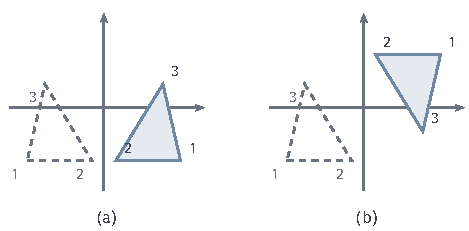
\includegraphics{figures/02-vectors-matrices-and-multivariate-calculus/03-linear-equations-and-optimization/tikz/learning-mechanisms/reflection-versus-rotation.pdf}
  \caption{反射与旋转的几何区别。虚线为原三角形，实色为变换后的位置；(a)关于纵轴反射，行列式为$-1$；(b)绕两轴交点旋转$180^\circ$，行列式为$1$。两幅图仅用于说明允许变换集合的不同，不表示给定矩阵的最优逼近结果。}
  \label{fig:solver-reflection-versus-rotation}
\end{figure}

\paragraph{$s=-1$时原来的上界取不到}
若$s=-1$，$\bm U\bm V^\top$不可行，需要新的上界。仍令$\bm Z=\bm U^\top\bm R\bm V$。对任一旋转$\bm R$，$\bm Z$正交，且
\[
 \det\bm Z=\det\bm U\cdot\det\bm R\cdot\det\bm V=s=-1 .
\]
上一小节的上界依赖$\bm Z=\bm I$可以取到；现在$\det\bm I=1$，这已不可能。

先看$d=2$。行列式为$-1$的二阶正交矩阵都形如
\[
 \bm Z=\begin{bmatrix}\cos\theta&\sin\theta\\\sin\theta&-\cos\theta\end{bmatrix},
\]
它是关于一条直线的反射。代入上一小节的目标，
\[
 \operatorname{tr}(\bm Z^\top\bm\Sigma)=\sigma_1\cos\theta-\sigma_2\cos\theta=(\sigma_1-\sigma_2)\cos\theta .
\]
由$\sigma_1\geq\sigma_2$，它在$\theta=0$处取最大值$\sigma_1-\sigma_2$，这时
\[
 \bm Z=\begin{bmatrix}1&0\\0&-1\end{bmatrix}.
\]
与无约束的上界$\sigma_1+\sigma_2$相比，迹少了$2\sigma_2$：两个对角元不能都取$1$，较小奇异值对应的那个对角元被迫取$-1$。这个例子中$\operatorname{tr}\bm Z=0=d-2$，下面的引理说明一般情形也如此。

\begin{lemma}[行列式为负的正交矩阵的迹]
\label{lem:matrix-approximation-reflection-trace}
设$\bm Z\in\mathbb R^{d\times d}$正交且$\det\bm Z=-1$，则存在单位向量$\bm x$使$\bm Z\bm x=-\bm x$，并且$\operatorname{tr}\bm Z\leq d-2$。
\end{lemma}
\begin{proof}
先证$-1$是特征值。由$\bm Z^\top\bm Z=\bm I$，
\[
 \bm Z+\bm I=\bm Z(\bm I+\bm Z^\top)=\bm Z(\bm I+\bm Z)^\top .
\]
取行列式得
\[
 \det(\bm Z+\bm I)=\det\bm Z\cdot\det(\bm I+\bm Z)=-\det(\bm Z+\bm I),
\]
所以$\det(\bm Z+\bm I)=0$，存在单位向量$\bm x$使$\bm Z\bm x=-\bm x$。再由
\[
 \bm x=\bm Z^\top\bm Z\bm x=-\bm Z^\top\bm x
\]
得$\bm Z^\top\bm x=-\bm x$。

$d=1$时$\bm Z=(-1)$，$\operatorname{tr}\bm Z=-1=d-2$。设$d\geq2$，把$\bm x$扩充为$\mathbb R^d$的标准正交基，排成正交矩阵$\bm Q=[\bm x,\bm Q_2]$。由$\bm Z\bm x=-\bm x$与$\bm Z^\top\bm x=-\bm x$，非对角块为零：
\[
 \bm Q_2^\top\bm Z\bm x=-\bm Q_2^\top\bm x=\bm0,\qquad
 \bm x^\top\bm Z\bm Q_2=(\bm Z^\top\bm x)^\top\bm Q_2=\bm0 .
\]
于是
\[
 \bm Q^\top\bm Z\bm Q=\begin{bmatrix}-1&\bm0\\\bm0&\bm Z_2\end{bmatrix},\qquad\bm Z_2=\bm Q_2^\top\bm Z\bm Q_2 .
\]
左端是正交矩阵的乘积，仍正交，所以$\bm Z_2$的各列是单位向量，对角元都不超过$1$，$\operatorname{tr}\bm Z_2\leq d-1$。迹在相似变换下不变，故
\[
 \operatorname{tr}\bm Z=-1+\operatorname{tr}\bm Z_2\leq d-2 .
\]
\end{proof}

用特征值的语言看，同一结论是这样的。实正交矩阵的特征值模都为$1$：非实特征值成共轭对出现，每对的乘积为$1$、实部之和不超过$2$；实特征值只能是$\pm1$。行列式等于全部特征值之积，为$-1$时特征值$-1$必出现奇数次，至少一次。迹等于特征值之和，于是至多为$(d-1)\cdot1+(-1)=d-2$。上面的证明只用实向量完成了同一论证。

\paragraph{修正最小奇异方向}
有了引理，就可以像$d=2$时那样估计迹的损失。把无约束上界与目标相减，
\[
 \sum_{i=1}^d\sigma_i-\operatorname{tr}(\bm Z^\top\bm\Sigma)=\sum_{i=1}^d\sigma_i(1-z_{i,i}).
\]
每个$1-z_{i,i}$都非负，由引理，它们的和是$d-\operatorname{tr}\bm Z\geq2$。损失是这些量以奇异值为权重的和，而每个权重都不小于最小奇异值$\sigma_d$，所以损失至少是
\[
 \sigma_d(d-\operatorname{tr}\bm Z)\geq2\sigma_d .
\]
这个下界在缺口全部集中于最后一个对角元时取到：$z_{d,d}=-1$，$1-z_{d,d}=2$，其余对角元都等于$1$。相应的$\bm Z$是
\begin{equation}
 \bm D_s=\operatorname{diag}(1,\ldots,1,s),
 \label{eq:matrix-approximation-rotation-correction}
\end{equation}
即只把最后一个对角元改为$s=-1$。换回原变量，最优旋转是$\bm R_\star=\bm U\bm D_s\bm V^\top$。$s=1$时$\bm D_s=\bm I$，这个公式也包含了行列式约束不起作用的情形。

\begin{theorem}[最佳旋转逼近]
\label{thm:matrix-approximation-best-rotation}
设$\bm A\in\mathbb R^{d\times d}$有SVD$\bm A=\bm U\bm\Sigma\bm V^\top$，$\sigma_1\geq\cdots\geq\sigma_d\geq0$，$s=\det(\bm U\bm V^\top)$，$\bm D_s=\operatorname{diag}(1,\ldots,1,s)$。则对一切满足$\bm R^\top\bm R=\bm I$、$\det\bm R=1$的$\bm R$，
\begin{equation}
 \operatorname{tr}(\bm R^\top\bm A)\leq\sum_{i=1}^{d-1}\sigma_i+s\,\sigma_d ,
 \label{eq:matrix-approximation-rotation-trace-bound}
\end{equation}
等号由$\bm R_\star=\bm U\bm D_s\bm V^\top$取到。因此
\begin{equation}
 \min_{\bm R^\top\bm R=\bm I,\ \det\bm R=1}\lVert\bm A-\bm R\rVert_{\mathrm F}^2
 =\sum_{i=1}^{d-1}(\sigma_i-1)^2+(\sigma_d-s)^2 .
 \label{eq:matrix-approximation-rotation-min-error}
\end{equation}
\end{theorem}
\begin{proof}
$\bm R_\star$是正交矩阵的乘积，仍正交，且$\det\bm R_\star=\det\bm U\cdot s\cdot\det\bm V=s^2=1$，所以它是旋转。

$s=1$时$\bm D_s=\bm I$，上界就是定理~\ref{thm:ls-best-orthogonal-approximation}对全部正交矩阵给出的$\sum_i\sigma_i$，在旋转中自然成立，且由$\bm R_\star=\bm U\bm V^\top$取到。

设$s=-1$。对任一旋转$\bm R$，令$\bm Z=\bm U^\top\bm R\bm V$，则$\det\bm Z=-1$，由引理~\ref{lem:matrix-approximation-reflection-trace}，$\operatorname{tr}\bm Z\leq d-2$。与上一小节相同，$\operatorname{tr}(\bm R^\top\bm A)=\sum_i\sigma_iz_{i,i}$。由$|z_{i,i}|\leq1$得$1-z_{i,i}\geq0$，又$\sigma_i\geq\sigma_d$，所以
\[
 \begin{aligned}
 \sum_{i=1}^d\sigma_i-\operatorname{tr}(\bm R^\top\bm A)
 &=\sum_{i=1}^d\sigma_i(1-z_{i,i})
 \geq\sigma_d\sum_{i=1}^d(1-z_{i,i})\\
 &=\sigma_d(d-\operatorname{tr}\bm Z)\geq2\sigma_d ,
 \end{aligned}
\]
即
\[
 \operatorname{tr}(\bm R^\top\bm A)\leq\sum_{i=1}^{d-1}\sigma_i-\sigma_d .
\]
$\bm R=\bm R_\star$时$\bm Z=\bm D_s$，迹恰为$\sum_{i<d}\sigma_i-\sigma_d$，等号成立。

最后代入展开式。由$\lVert\bm A\rVert_{\mathrm F}^2=\sum_i\sigma_i^2$与$s^2=1$，
\[
 \sum_{i=1}^d\sigma_i^2+d-2\Bigl(\sum_{i=1}^{d-1}\sigma_i+s\sigma_d\Bigr)
 =\sum_{i=1}^{d-1}(\sigma_i-1)^2+(\sigma_d-s)^2 .
\]
\end{proof}

\paragraph{修正的代价}
修正只发生在最小奇异方向上。$\bm R_\star=\bm U\bm D_s\bm V^\top$与无约束解$\bm U\bm V^\top$的差别，是把最后一对奇异方向的配对改为$\bm v_d\mapsto s\bm u_d$。若把符号改放在第$i$个方向上，同样得到旋转，但迹损失$2\sigma_i$；定理证明中的不等式说明，任何旋转的迹损失都至少是$2\sigma_d$，所以放在最小奇异方向上损失最少。

$s=-1$时，最小平方误差比无行列式约束时增加
\begin{equation}
 (\sigma_d+1)^2-(\sigma_d-1)^2=4\sigma_d .
 \label{eq:matrix-approximation-rotation-cost}
\end{equation}
$\bm A$可逆时，$\det\bm A=\det\bm U\det\bm\Sigma\det\bm V$且$\det\bm\Sigma>0$，所以$s$就是$\det\bm A$的符号，与所取的SVD无关：$\det\bm A>0$时约束不起作用，$\det\bm A<0$时代价为$4\sigma_d$。

$\sigma_d=0$时，$s$依赖SVD的选取：把$\bm u_d$换成$-\bm u_d$不改变$\bm A$，却改变$\det\bm U$的符号。但这时$(\sigma_d-s)^2=1$与$s$无关，旋转约束的代价为零。两种选取还给出同一个$\bm R_\star$，因为符号同时出现在$\bm u_d$与$s$中，乘积$s\bm u_d$不变。

\paragraph{唯一性}
唯一性分两种情形说明。第一种，$\bm A$可逆且$s=1$：无约束问题的唯一解$\bm W$本身是旋转，所以它也是旋转约束下的唯一解。

第二种，$\sigma_{d-1}>\sigma_d$。若$\sigma_d>0$且$s=-1$，定理证明中的不等式取等要求$(\sigma_i-\sigma_d)(1-z_{i,i})=0$，从而$i<d$时$z_{i,i}=1$，$\bm Z$的前$d-1$列是$\bm e_1,\ldots,\bm e_{d-1}$；最后一列只能是$\pm\bm e_d$，行列式为$-1$又迫使它为$-\bm e_d$，即$\bm Z=\bm D_s$。

若$\sigma_d=0$，先取使$s=1$的SVD，取等要求$z_{i,i}=1$（$i<d$），同理$\bm Z=\operatorname{diag}(1,\ldots,1,\pm1)$，而$\det\bm Z=s=1$，故$\bm Z=\bm I$。两种情况下最优旋转都唯一。

最小奇异值重复且$s=-1$，或$\operatorname{rank}\bm A\leq d-2$时，最优旋转可以不唯一，例子见本小节的算法分析。

\subsubsection{算法实现}

计算在上一小节的基础上增加两步：求出符号$s$，再在最小奇异方向上作修正。下面写出用到的变量与各步计算，并用以下示例逐步演示。

\begin{example}[对角矩阵的旋转逼近]
\label{ex:matrix-approximation-rotation-diagonal}
求离
\[
 \bm A=\begin{bmatrix}3&0\\0&-1\end{bmatrix}
\]
最近的旋转。$\det\bm A=-3<0$，上一小节的无约束解包含反射，行列式约束会起作用。下面的逐步执行给出$\bm R_\star$与平方误差，并与无约束解比较。
\end{example}

\paragraph{变量}
\begin{itemize}
 \item $\bm A\in\mathbb R^{d\times d}$：给定的方阵。
 \item $\bm U,\bm\Sigma,\bm V$：$\bm A$的完整方阵SVD，奇异值按非增顺序排列。
 \item $s=\det\bm U\det\bm V$：无约束解$\bm U\bm V^\top$的行列式。
 \item $\bm D_s=\operatorname{diag}(1,\ldots,1,s)$：最小奇异方向上的符号修正。
 \item $\bm R_\star$：所求的最优旋转。
\end{itemize}

\paragraph{输入与预处理}
输入方阵$\bm A$，预处理是求它的完整方阵SVD，并把奇异值按非增顺序排列，使最后一列$\bm u_d$、$\bm v_d$对应最小奇异值。符号修正要放在这一对方向上，排序不能省略。

例中
\[
 \bm A^\top\bm A=\begin{bmatrix}9&0\\0&1\end{bmatrix},
\]
可取$\bm V=\bm I$，奇异值$\sigma_1=3\geq\sigma_2=1$。由$\bm u_i=\bm A\bm v_i/\sigma_i$，
\[
 \bm u_1=\frac13\begin{bmatrix}3\\0\end{bmatrix}=\begin{bmatrix}1\\0\end{bmatrix},\qquad
 \bm u_2=\frac11\begin{bmatrix}0\\-1\end{bmatrix}=\begin{bmatrix}0\\-1\end{bmatrix},
\]
于是
\[
 \bm U=\begin{bmatrix}1&0\\0&-1\end{bmatrix},\qquad
 \bm\Sigma=\begin{bmatrix}3&0\\0&1\end{bmatrix},\qquad
 \bm V=\bm I ,
\]
核对$\bm U\bm\Sigma\bm V^\top=\operatorname{diag}(3,-1)=\bm A$。

\paragraph{计算步骤}
\begin{enumerate}
 \item \textbf{计算符号。}按式~\eqref{eq:matrix-approximation-rotation-sign}计算
 \[
  s=\det\bm U\det\bm V .
 \]
 例中
 \[
  s=(-1)\cdot1=-1 .
 \]
 作为对照，无约束的最优正交矩阵是$\bm U\bm V^\top=\operatorname{diag}(1,-1)$，它是关于横轴的反射，平方误差为
 \[
  \lVert\operatorname{diag}(2,0)\rVert_{\mathrm F}^2=4=(3-1)^2+(1-1)^2 .
 \]

 \item \textbf{构造修正矩阵。}按式~\eqref{eq:matrix-approximation-rotation-correction}取
 \[
  \bm D_s=\operatorname{diag}(1,\ldots,1,s).
 \]
 例中
 \[
  \bm D_s=\begin{bmatrix}1&0\\0&-1\end{bmatrix}.
 \]

 \item \textbf{相乘得最优旋转。}计算
 \begin{equation}
  \bm R_\star=\bm U\bm D_s\bm V^\top .
  \label{eq:matrix-approximation-rotation-optimum}
 \end{equation}
 例中
 \[
  \bm R_\star=\begin{bmatrix}1&0\\0&-1\end{bmatrix}\begin{bmatrix}1&0\\0&-1\end{bmatrix}=\begin{bmatrix}1&0\\0&1\end{bmatrix}.
 \]

 \item \textbf{核验。}同时检查三项：$\bm R_\star^\top\bm R_\star=\bm I$，$\det\bm R_\star=1$，误差平方等于$\sum_{i<d}(\sigma_i-1)^2+(\sigma_d-s)^2$。

 例中$\bm R_\star=\bm I$，前两项显然成立；残差为$\bm A-\bm R_\star=\operatorname{diag}(2,-2)$，
 \[
  \lVert\bm A-\bm R_\star\rVert_{\mathrm F}^2=4+4=8=(3-1)^2+(1+1)^2 .
 \]
 比无约束时多$4=4\sigma_2$。
\end{enumerate}

最终得到离$\bm A$最近的旋转
\[
 \bm R_\star=\begin{bmatrix}1&0\\0&1\end{bmatrix},
\]
平方误差为$8$。

二阶旋转可以全部写出来，用于独立核对。对
\[
 \bm R=\begin{bmatrix}\cos\theta&-\sin\theta\\\sin\theta&\cos\theta\end{bmatrix},
\]
按元素求和得
\[
 \operatorname{tr}(\bm R^\top\bm A)=3\cos\theta-\cos\theta=2\cos\theta ,
\]
它只在$\theta=0$处取最大值$2=\sigma_1-\sigma_2$。所以$\bm R_\star=\bm I$是唯一的最优旋转，与$\sigma_1>\sigma_2$时的唯一性一致。

\subsubsection{算法分析}

\paragraph{计算代价}
与无约束情形相比，额外的工作只是求两个正交矩阵的行列式与一次对角缩放，主要代价仍是SVD。是否需要修正完全由$s$决定，不必比较多个候选。

\paragraph{最优旋转不唯一的情形}
最小奇异值重复时，唯一性可能失败。取$\bm A=\operatorname{diag}(1,-1)$，奇异值为$1,1$，$s=-1$。对上面的任一二阶旋转，
\[
 \operatorname{tr}(\bm R^\top\bm A)=\cos\theta-\cos\theta=0 ,
\]
由展开式~\eqref{eq:matrix-approximation-orthogonal-expansion}，所有旋转的误差平方都是
\[
 \lVert\bm A\rVert_{\mathrm F}^2+2-0=4 ,
\]
与公式$(1-1)^2+(1+1)^2=4$一致，但最优旋转有无穷多个。

$\operatorname{rank}\bm A\leq d-2$时也有类似的自由度，例如$\bm A=\bm0$时每个旋转都最优。

\paragraph{接近奇异时的敏感性}
最小奇异值接近零时，$s$对$\bm A$的微小变化很敏感：$\det\bm A$接近零，它的符号可能被扰动改变，最优旋转随之跳到另一个。但对同一个$\bm A$，两种符号给出的误差平方恰好相差$4\sigma_d$，这时也很小，最优误差本身随$\bm A$连续变化。所以这种情形下应报告最优误差，而不应把所得的旋转当作稳定的估计。

% 第15章第6节：逼近结果的检验。

\section{逼近结果的检验}
\label{sec:matrix-approximation-verification}

前几节的最优解都由SVD读出，实际计算出的近似矩阵还要检验。检验回答三个问题：结果是否满足约束，残差是否达到理论下界，残差中哪一部分来自约束本身、哪一部分来自计算。三项检验都要用问题所规定的那一种误差范数；用别的范数评价，会把正确的结果误判为不好，或把不好的结果误判为可接受。

第一项是约束。低秩近似若以因子$\bm U_k$、$\bm\Sigma_k$、$\bm V_k$的形式保存，秩不超过$k$由因子形式直接保证；若已经乘成完整矩阵$\widehat{\bm X}$，可以看它第$k$个以后的奇异值是否只在舍入误差的量级。正交逼近与旋转逼近要检查$\lVert\widehat{\bm R}^\top\widehat{\bm R}-\bm I\rVert_{\mathrm F}$是否接近零；旋转还要检查$\det\widehat{\bm R}=1$，而不是$-1$。

第二项是残差与理论下界的比较。直接计算残差，再与本章给出的最优误差对照：秩$k$逼近在Frobenius范数下为$(\sum_{i>k}\sigma_i^2)^{1/2}$，在谱范数下为$\sigma_{k+1}$；可分离权重下为$(\sum_{i>k}\tilde\sigma_i^2)^{1/2}$；正交逼近的平方误差为$\sum_i(\sigma_i-1)^2$，旋转逼近再加上$s=-1$时的$4\sigma_d$。

满足约束的任何候选，残差都不会低于这些下界。所以若直接算出的残差明显低于下界，说明结果实际上违反了约束（例如数值秩大于$k$），或者所用的奇异值本身不准确；若明显高于下界，则说明计算或截断有误，例如奇异值没有按降序排列，或左右奇异向量的配对被打乱。加权问题要用加权残差比较：示例~\ref{ex:matrix-approximation-weighted-low-rank}中的$\bm X_1=\operatorname{diag}(0,2)$按普通Frobenius范数的误差为$3$，比直接截断$\bm A$的误差$2$大，但它在加权意义下才是最优的。

第三项是区分两种误差。逼近误差由约束决定：秩预算或正交性使$\bm A$本身不可行时，即使精确计算，残差也等于理论下界而不为零，这部分不能靠提高计算精度消除。计算误差则是计算结果与精确最优解之间的差别，来自SVD等步骤的舍入，表现为直接残差与理论下界之间的差距，以及约束检验中偏离零的量。

两者对扰动的反应也不同。由第~\ref{chap:condition-and-spectral-perturbation}章奇异值的Weyl界（定理~\ref{thm:ls-weyl-singular-value}），$\bm A$受到谱范数不超过$\varepsilon$的扰动时，每个奇异值的变化不超过$\varepsilon$，所以最优误差$\sigma_{k+1}$的数值是稳定的。取得最优误差的矩阵却依赖奇异子空间：间隙$\sigma_k-\sigma_{k+1}$很小时，前$k$个奇异方向可能明显转动；间隙为零时，第~\ref{sec:matrix-approximation-low-rank-uniqueness}节已经说明最优矩阵本身不唯一。因此间隙很小时，应把最优误差当作可靠的结论，而把具体的近似矩阵当作许多近乎同样好的候选之一。

本章的算例可以按这三项核对。示例~\ref{ex:matrix-approximation-truncated-three-by-three}中$\bm A_1$秩为一，直接算出的残差为$\sqrt2$（Frobenius）与$1$（谱范数），分别等于$(\sigma_2^2+\sigma_3^2)^{1/2}$与$\sigma_2$；示例~\ref{ex:matrix-approximation-orthogonal-two-by-two}中$\bm R_\star^\top\bm R_\star=\bm I$，平方误差$5=(3-1)^2+(2-1)^2$；示例~\ref{ex:matrix-approximation-rotation-diagonal}中$\det\bm R_\star=1$，平方误差$8=4+4\sigma_2$。这些都是精确算例，计算误差为零，残差全部来自约束。

最后区分本章的截断与第~\ref{chap:solution-error-regularization}章的截断。那里的截断SVD求解$\bm x_k=\bm A_k^\dagger\bm b$同样只保留前$k$个奇异方向，但目的是从带误差的观测中稳定地求出输入，检验的是向量残差$\bm b-\bm A\bm x_k$与解的误差；选择$k$时，要同时比较舍弃方向带来的拟合损失与保留方向上$1/\sigma_k$的噪声放大。本章检验的是矩阵残差$\bm A-\bm A_k$，最佳矩阵逼近本身不替代那里对$k$的判断。

\FloatBarrier
\section{本章小结}
\label{sec:matrix-approximation-summary}

本章开头的问题是：给定矩阵$\bm A$，在秩约束或正交约束下，哪一个矩阵离它最近，最小误差是多少，最优矩阵是否唯一。各节的解法遵循同一条路线：先写清约束与误差；再固定一个表示，在其中选出最优系数；最后选择表示本身，即方向、子空间或正交因子。前两步把矩阵优化化成向量的投影与特征值比较，SVD则把最优解写成具体的矩阵。

秩一逼近中，固定单位方向$\bm u$时，最优系数是投影系数$\bm c=\bm A^\top\bm u$，误差等于$\lVert\bm A\rVert_{\mathrm F}^2$减去保留量$\bm u^\top\bm A\bm A^\top\bm u$。选方向就是最大化Rayleigh商。对任意实对称$\bm S$，Rayleigh商介于最小、最大特征值之间，取等的方向恰是相应特征空间中的非零向量。用到$\bm A\bm A^\top$上，最优秩一近似为$\sigma_1\bm u_1\bm v_1^\top$，平方误差为$\sum_{i\geq2}\sigma_i^2$；它在$\sigma_1>\sigma_2$时唯一，奇异向量同时变号只改变写法。

秩$k$逼近中，固定子空间的最优重建是正交投影，选子空间化为迹极值：$k$维子空间上的迹不超过前$k$个特征值之和。由此得到Eckart--Young--Mirsky定理：截断SVD$\bm A_k$在全部秩不超过$k$的矩阵中同时使Frobenius误差与谱范数误差最小，最小值分别为$(\sum_{i>k}\sigma_i^2)^{1/2}$与$\sigma_{k+1}$。Frobenius最优解在$\sigma_k>\sigma_{k+1}$时唯一；谱范数最优解即使有间隙也一般不唯一。这些结论只对全部秩不超过$k$的矩阵与这两种范数成立，额外的非负、稀疏约束或一般的逐元素权重都会使截断SVD失去最优性。

改用加权长度规定单位方向时，Rayleigh商推广为广义Rayleigh商。$\bm B$正定时，用Gram因子换元可化为普通Rayleigh商，极值是广义特征值，广义特征向量可以选成$\bm B$正交；计算用Cholesky分解与三角求解保持对称结构，不应改求一般不对称的$\bm B^{-1}\bm S$。$\bm B$不正定时这一化归失效。

误差的权重能分离为行权重与列权重时，加权低秩逼近经可逆变换化为普通低秩逼近，最优解由变换后矩阵的截断SVD还原，最佳方向正是一个广义Rayleigh商的最大特征向量。这一化归要求逐元素权重是行因子与列因子的乘积；任意权重与缺失元素没有截断SVD式的闭式解，交由卷五的优化方法处理。

正交约束下，距离最小化成迹最大化，目标关于未知矩阵是线性的。最优正交矩阵是$\bm U\bm V^\top$，即第~\ref{chap:polar-decomposition}章极分解的正交因子，平方误差为$\sum_i(\sigma_i-1)^2$；$\bm A$可逆时它唯一，奇异时自由度只在零奇异值方向上。要求旋转时，只需在最小奇异方向上作符号修正，$\bm R_\star=\bm U\operatorname{diag}(1,\ldots,1,\det(\bm U\bm V^\top))\bm V^\top$；$\det(\bm U\bm V^\top)=-1$时误差平方增加$4\sigma_d$，$\sigma_d=0$时修正不增加误差。

在这些问题中，Rayleigh商、迹极值与截断SVD承担的是最优性工具的职责：它们说明为什么由SVD读出的矩阵最好，以及在什么条件下唯一。计算出的结果要按同一种误差范数检验约束与残差，把约束带来的逼近误差与计算误差分开；最优误差的数值对扰动稳定，最优矩阵在间隙小时则不稳定。本章的截断矩阵用于重建$\bm A$本身，与第~\ref{chap:solution-error-regularization}章为稳定求解方程而截断取逆的用途不同；不能化归到SVD的一般逼近问题，则由卷五的迭代优化展开。

